\section{Information-Driven Exploration}

\begin{figure}
\centering
\begin{tabular}{cc}
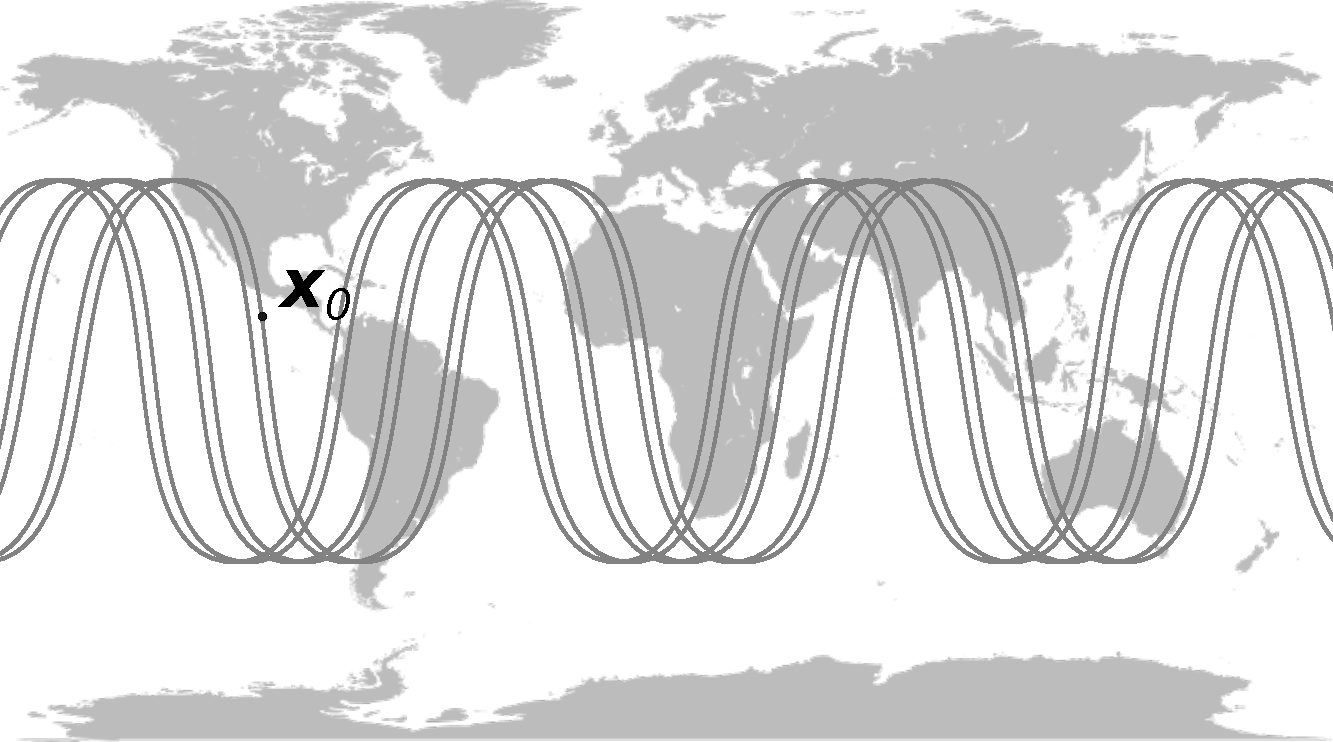
\includegraphics[height=1.5in]{world_map} &
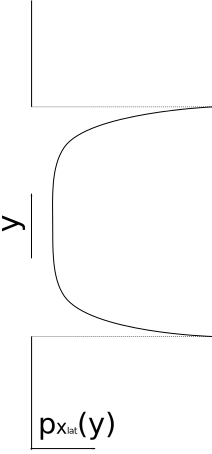
\includegraphics[height=1.5in]{world_map_belief}
\\
\tiny{\texttt{https://upload.wikimedia.org/wikipedia/commons/e/ec/World\_map\_blank\_without\_borders.svg}}
\end{tabular}
\caption{\emph{Lost Astronaut Prior Distribution}
The crash site $\x(t)$ is defined by a random time $t$, chosen uniformly in $[0,T]$.
This induces prior marginal probabilities on the latitude and longitude of the crash site.
The limiting distribution for as $T\to\infty$ is shown at right, while the limiting distribution
on longitude is uniform.
}
\label{fig: lost astronaut}
\end{figure}

\begin{figure}
\centering
\subfigure[Freely-placed obstacles]{
\begin{tabular}{c}
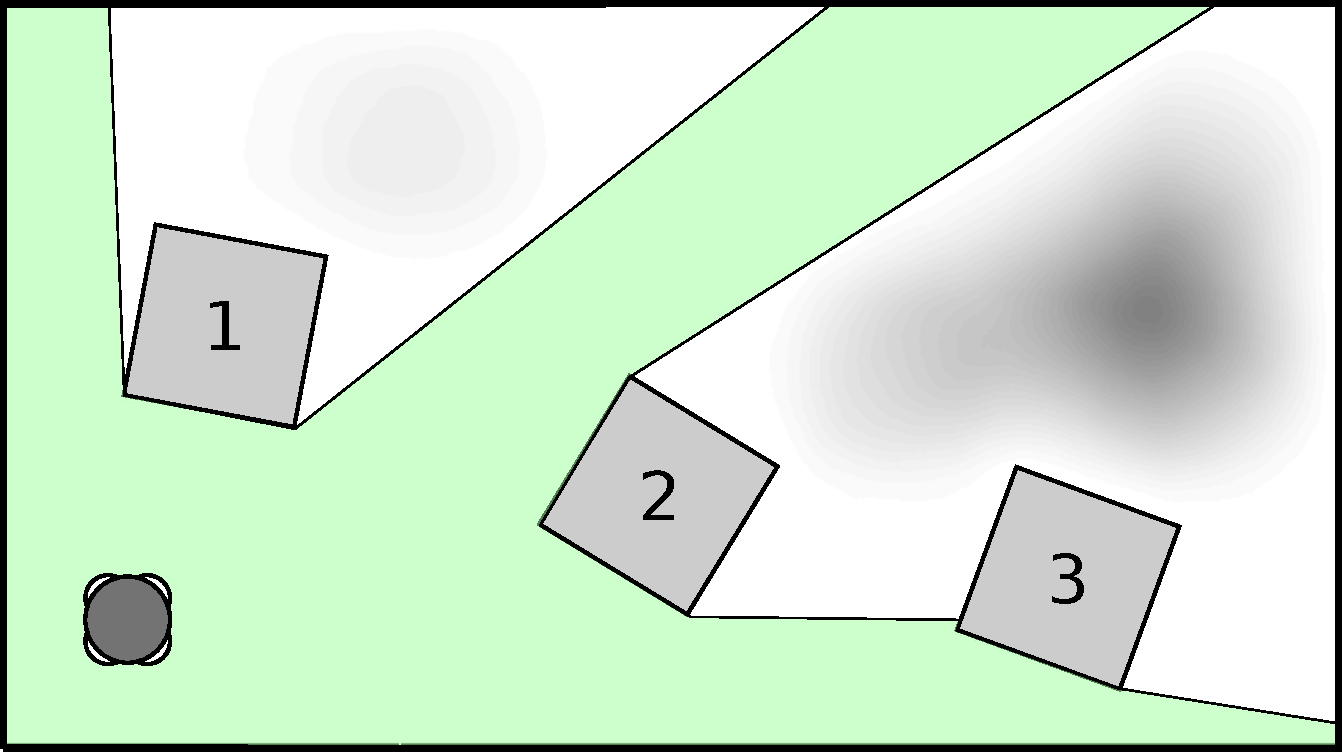
\includegraphics[height=1in]{random_block_marg}\\
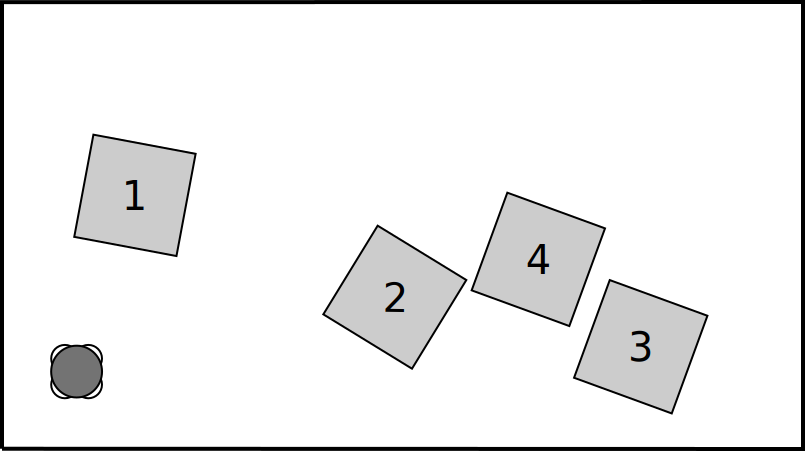
\includegraphics[height=1in]{random_block}
\end{tabular}\qquad
}
\subfigure[Gridded obstacles]{
\begin{tabular}{c}
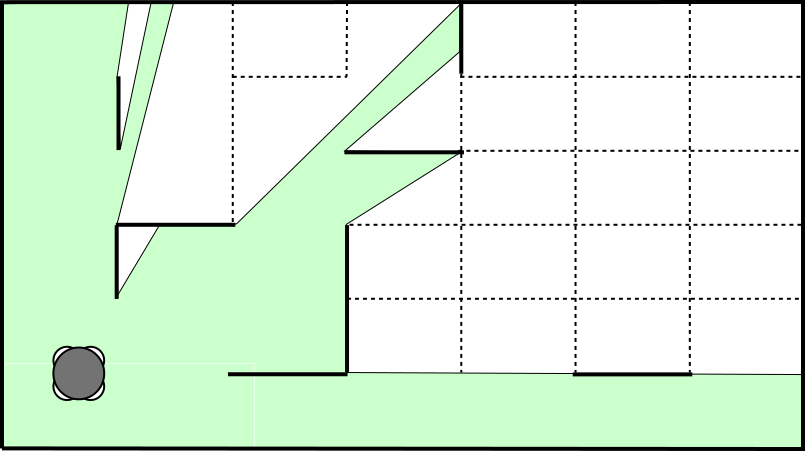
\includegraphics[height=1in]{random_room_belief}\\
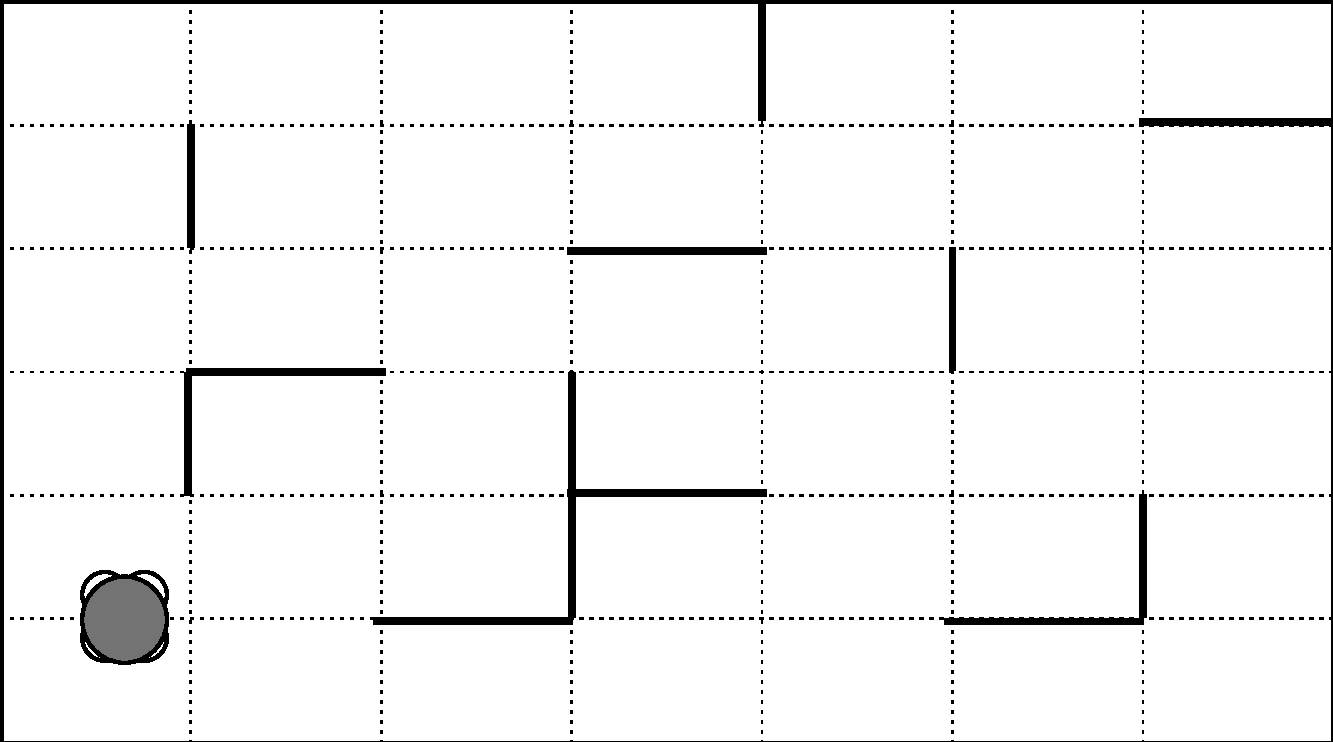
\includegraphics[height=1in]{random_room}
\end{tabular}
}
\caption{\emph{Exploring a Random Room}
(a) In the first case, the explorer knows that 
there are four identical boxes scattered within a
room of known dimensions, three of which he can see.
There is a ``shadow region'' where the disposition of 
space is not known.  Based on allowable configurations 
of the missing block (blocks can not intersect, 
unseen blocks can not lie in known free space), the
explorer can compute, at each point in the shadow region,
the probability that that point is covered by an obstacle.
(b) In the second case, partitions (black line segments),
constrained to grid lines (dotted lines)
divide up a room.  Seeing any point of a grid segment
reveals the disposition of any other point on that grid segment.
}
\end{figure}

\begin{figure}
\centering
\subfigure[First View]{
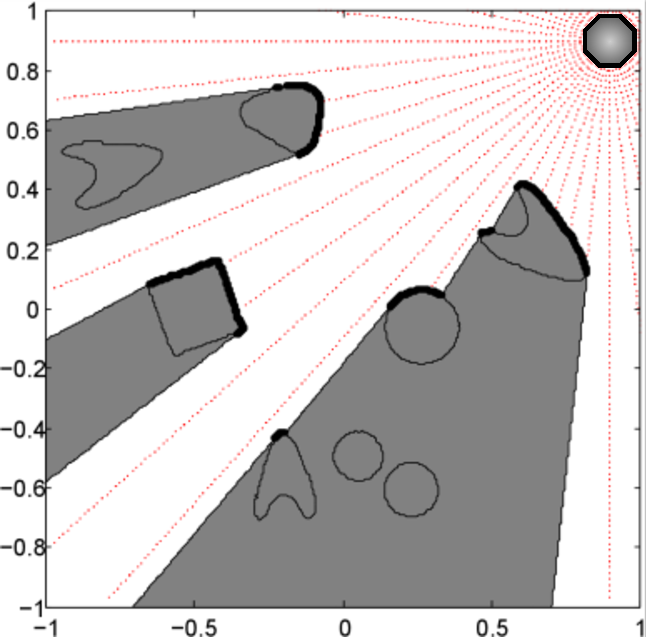
\includegraphics[width=1.5in]{first_view.pdf}}
\subfigure[New Vantage Point]{
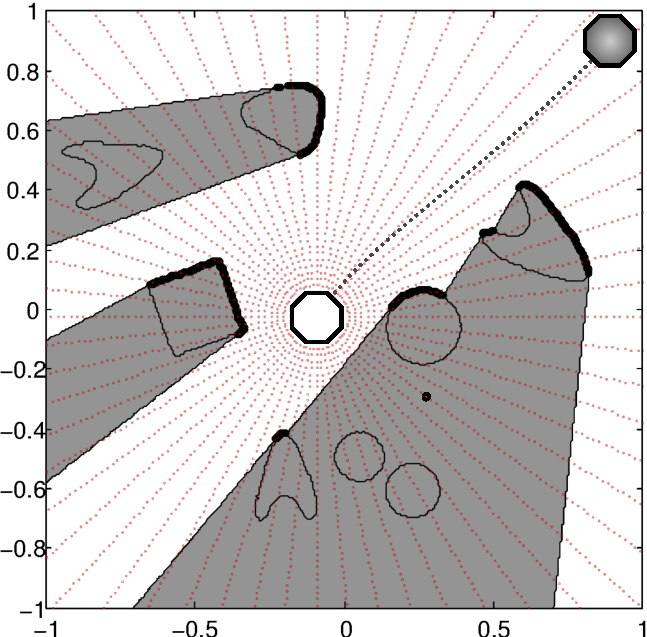
\includegraphics[width=1.5in]{first_hypoth.pdf}}
\subfigure[Hypoth.\ Second View]{
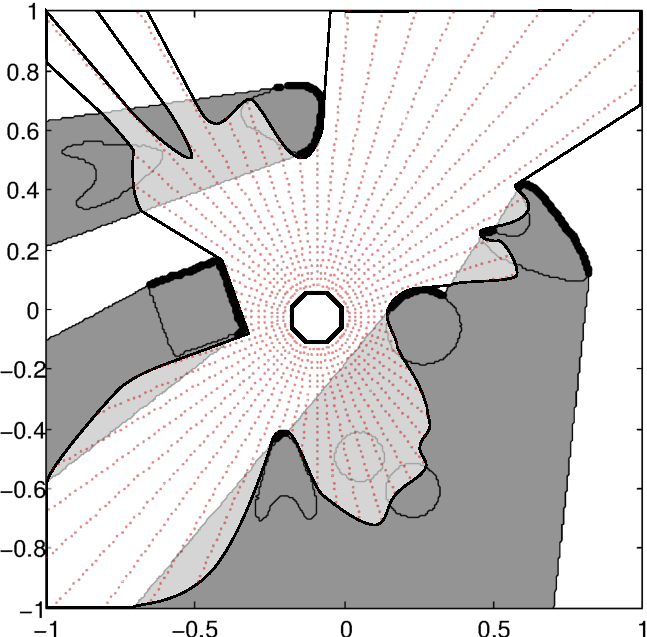
\includegraphics[width=1.5in]{first_meas.pdf}}
\caption{\emph{Range Measurement Planning} An explorer \label{fig: grids}}
\end{figure}
In this chapter we consider the problem where the
variable of interest is the geometry and topology of a
two-dimensional scene (e.g. the map of a building) 
represented by an indicator function defined on a domain
$\Omega \subs \RR^2$, supported on a closed subset
$\O \subs \Omega$ that describes unknown ``obstacles'' or ``objects.''
The explorer follows a continuous path $x(t)$
in the space $\Omega\andn\O$.
Let $\A \subs \Omega \andn \O$ be
the path-component of $\Omega \andn \O$ containing $x(0)$.

At discrete timesteps $t_i$, $i=1, \ldots, L$, the explorer at $x_i = x(t_i)$ measures an 
$n$-directional range map $\Y(x_i) \in (s\NN)^n$, % $\ZZ_n\to s\NN$,
which gives, to the nearest multiple of $s>0$, the distance 
to the first obstacle along each sensor element's line of sight.  
Let $\Y^t = \{\Y(x_i)\,:\;t_i<t\}$ denote the history of  measurements up to time $t$.  

Observe that each measurement is a
function $\Y(x) = h(x, \Omega, \O)$ of the scene $(\Omega, \O)$ and the vantage point $x$.
%(we will sometimes write $\Y(x)$ to highlight that
%a measurement $\Y$ was taken at the point $x$).
If we interpret
this as a realization of a stochastic process, each measurement
$\Y_i$ reduces the uncertainty in $\O$. Although each
range sensor is affected by uncertainty due to scaling,
spatial quantization, noise, etc. most of the uncertainty
is due to occlusions, for objects are opaque and therefore 
at the outset we have no knowledge of the scene behind 
an occluder. An information-gathering controller
then aims to design the control $\{u_j\}_{j=i}^L$ that maximizes
the reduction in the entropy of $\O$. Here we will assume
for simplicity that we can control the instantaneous 
velocity, so that $x_{i+1} = x_i + u_i$. 
%Of course, more complex vector fields can be employed, 
%but for the purpose of exposition we describe the state
%model as a simple integrator.

% and the \emph{visible region} $\A^t \subs \A$ as the region in $\A$ with an unobstructed view of some part of $\{x(\tau):\tau\leq t\}$.
%A range map $y$ at $x$ defines a star-shaped region:
%$R_x(y) := \{x\1\in \Omega: d(x,x\1) < y(\theta(x,x\1))\}$,
%where $\theta(x,x\1)\in\SS$ is the direction from point $x$ to point $x\1$.
In order to compute the “information gain” of a measurement at time $t$, we have
to define suitable distributions on the objects of 
interest. 
We maintain an estimate of the explorer's state at time $t$
as a distribution $\PP_t[\,\cdot\,] = \PP[\,\cdot\,|\Y^t\bigr]$ on possible realizations of $\A$.

\section{Next-View Entropy}


In order to compute the “information gain” of a measurement at time $t$, we have
to define suitable distributions on the objects of 
interest. 
We maintain an estimate of the explorer's state at time $t$
as a distribution $\PP_t[\,\cdot\,] = \PP[\,\cdot\,|\Y^t\bigr]$ on possible realizations of $\A$.
Let $\A_t = \{x\in \Omega\,:\, \PP_t[x\in\A] = 1\}$,
$\O_t = \{x\in \Omega\,:\, \PP_t[x\in\A] = 0\}$,
and $\U_t = x \andn (\A_t \cup \O_t)$
be the points which at time $t$ are 
known to be visible, known to be invisible, or unknown,
respectively.  Finally, let $\V^t$ denote the set of points that are visible to the observer from point $x_t$.

\subsection{Measurement Uncertainty}
Let 
$$G=\left\{g_{ij} := s\,i\bigl(\cos(2\pi j/n), \sin(2\pi j/n)\bigr)\right\}\substack{i,j\in\NN\\ j<n}$$
be a uniform radial grid, centered at the origin, with radial spacing $s$ and angular spacing $2\pi/n$
(see Figure \ref{fig: grids}).
Although we define $\Y(x) = h(x, \Omega, \O)$ as an $s\NN$-valued random $n$-tuple,  
%measuring the distance from $x$ to the nearest obstacle along $n$ lines of sight,
it is natural to define an ``alter-ego'' $\Y_G(x)$, 
a Boolean-valued random vector indexed by sample points $g_{ij}\in G$,
with the constraint that 
\begin{equation}
\Y_G(x)_{ij} = 0 \implies \Y_G(x)_{i+1, j}=0.
\footnote{This formalizes the notion that a visible object blocks the view of 
objects further along its line of sight.} \label{eq: ordering constraint}
\end{equation}
Let $\Y(x)_{ij}=1$ iff the point $g_{ij} + x$ is visible from $x$.
Observe that
$$\Y_G(x)_{ij} = \one\{\Y(x)_j < s\,i\}.$$
This defines a bijective relation between $\Y_G(x)$ and $\Y(x)$, so $\HH_t[\Y_G (x)] = \HH_t[\Y(x)]$.

Our next-view energy
$E_t(x)$ is the expected decrease in uncertainty at time $t$,
%$\HH_t\bigl[\O\bigr]$
%$\HH\bigl[\O|\Y^t\bigr]$ 
due to a measurement $\Y(x)$:
\begin{align*}
E_t(x) :&= \EE_t\bigl[\HH_t[\O] - \HH_t[\O|\Y(x)]\bigr] = \EE_t\bigl[\HH_t[\Y(x)]\bigr]\\
&= \HH_t[\Y(x)] = \HH_t[\Y_G(x)]. 
\intertext{
We can decompose the latter into a sum of relative entropies, 
given a ordering $g_{o_1}, g_{o_2}, \ldots$ on $G$ that respects radial ordering 
(i.e. if $o_k = (i,j)$, $o_\ell = (i\1, j\1)$, and $i\1<i$, then $\ell<k$):
}
&= \sum_k \HH_t\bigl[\Y_G(x)_{o_k}\,|\,\{\Y_G(x)_{o_{\ell}}\}_{\ell<k}\bigr].
\end{align*}
Now, if $\Y_G(x)_{i\1,j} = 0$ for $i\1<i$, then by (\ref{eq: ordering constraint}), 
we know $\Y(x)_{i,j}$ must equal 0 as well.
In that case, the relative entropy at $g_{ij}$ is zero, and so
\begin{align}
&=\sum_{o_k=(i,j)} \underset{\text{Probability that $x+g_{ij}$ is visible from $x$}}
{\underbrace{\PP_t\bigl[\Y_G(x)_{i\1j}=1\;\text{ for all $\;i\1<i$}\bigr]}}\notag\\
&\qquad\quad\cdot\;
\underset{\text{Value of revealing scene at $x+g_{ij}$}}
{\underbrace{\HH_t\bigl[\Y_G(x)_{o_k}\;|\;
\{\Y_G(x)_{o_{\ell}}\;|\;\ell<k\},\;
\Y_G(x)_{i\1j}=1\;\text{for all $\;i\1<i$}
\bigr]}}. \label{eq: king}
\end{align}
Here, we will reference the first term through its complement, 
which we will call the ``extinction probability''.
\subsubsection{Extinction Probability}
Define a normalized, instantaneous ``mean free path'' function 
$\operatorname{MFP}:\Omega\to[0,\infty)$, such that 
for any curve $C\subs\Omega$,
$$
\PP_t\bigl[C\in\A] = \exp\Biggl(\int_C
\frac{\log\bigl(\PP_t(x+g_{ij}\in\A)\bigr)}{\operatorname{MFP(y)}}|dy|\Biggr).
$$
Now we compute extinction probability, using a posterior estimate of the scene
\begin{align*}
\PP_t\bigl[\Y_G(x)_{ij}=1 \;|\; \Y_G(x)_{i-1,j}=1\big] 
&= \exp\Biggl(\underset{\!\!\!\mathrlap{\text{line}(x+g_{i-1,j},\,x+g_{ij})}}{\int}\; 
\frac{\log\bigl(\PP_t(x+g_{ij}\in\A)\bigr)}{\operatorname{MFP(y)}}|dy|\Biggr)\\
&\approx \PP_t(x+g_{ij}\in\A)^{s/\operatorname{MFP}(x+g_{ij})},
\end{align*}
Induction on this chain of conditional probabilities gives
$$\PP_t\bigl[\Y_G(x)_{ij}=1] \approx \prod_{i\1<i} \PP_t(x+g_{i\1j}\in\A)^{s/\operatorname{MFP}(x+g_{i\1j})}$$ 

\subsubsection{View Value}
The second term in (\ref{eq: king}) is a conditional entropy whose computation is only tractable in certain limited situations.
We will discuss these in the next section.

\section{Obstacle Models \label{section: obstacle models}}
\subsection{Uniform Obstacle Density}
The simplest obstacle model assigns, to all points in $\U^t$, 
equal and nonzero probability $p$ of lying in an obstacle.
Additionally, it treats each sampled point as independent of all others.
Thus the difficult entropy term in (\ref{eq: king}) reduces to a Bernoulli entropy:
\begin{align*}
&\HH_t\bigl[\Y_G(x)_{o_k=(i,j)}\;|\;
\{\Y_G(x)_{o_{\ell}}\;|\;\ell<k\},\;
\Y_G(x)_{i\1j}=1\;\text{for all $\;i\1<i$}
\bigr] = \HH_t\bigl[\Y_G(x)_k\bigr] \\
&\qquad=-p\log p - (1-p)\log p,
\end{align*}
where we take $0\log 0$ as 0.  Additionally, we treat $\operatorname{MFP}(y)$ as constant.
define 

\begin{align}
E_t(x)&=\sum_{ij} \bigl(-p_{ij}\log p_{ij} - (1-p_{ij})\log (1-p_{ij})\bigr) \prod_{i\1<i} p_{i\1j}^{s/\operatorname{MFP}},
\end{align}
where
$$p_{i,j} = \begin{cases}
0 & \operatorname{line}(x+g_{i-1,j}, x+g_{ij}) \cap \O^t \neq \emptyset \\
1 & \text{o.w, } x+g_{ij}\in\A^t\\
p & \text{o.w}
\end{cases}.$$
The values $p$ and $\operatorname{MFP}$ are model parameters.

\def\n{\vec{n}}
\begin{figure}
\centering
\subfigure[Low $p$]{
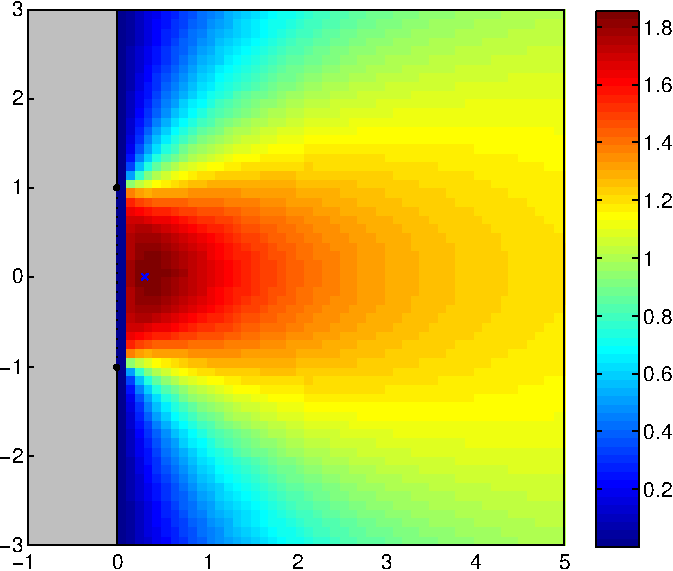
\includegraphics[height=1.3in]{JEnergy1}}
\subfigure[High $p$]{
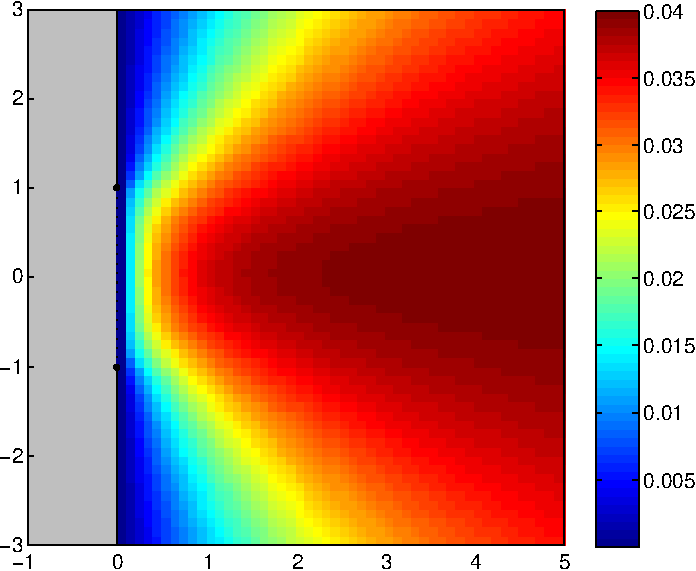
\includegraphics[height=1.3in]{JEnergy25}
}
\subfigure[View Penetration]{
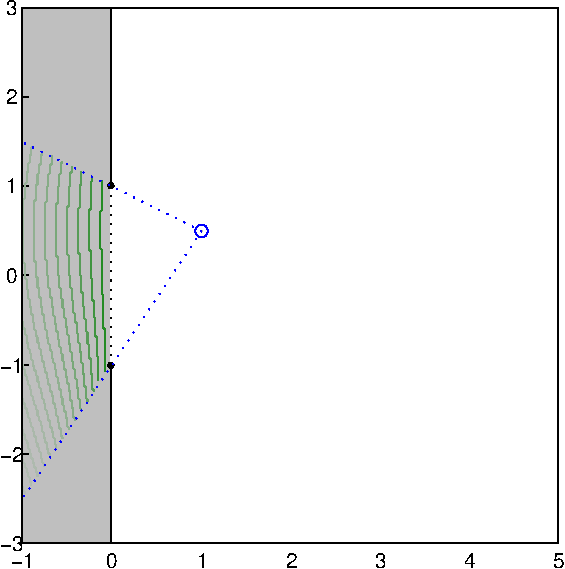
\includegraphics[height=1.3in]{penetration1}}
\caption{\emph{Looking into a Closet with Uniform Obstacle Density}
(a)-(b) Here we show the value of different vantage points
for looking into an unexplored closet, 
for various values of $p$ (MFP fixed).
As $p$ increases, a line of sight is less and less likely to 
penetrate deeply into the room, so the 
best vantage points move further back where 
lines of sight are more oblique.
(c) Green lines show the probability-0.5 penetration limits of
the blue explorer, for different values of $p$.  
As $p\to 1$, the depth of penetration near a point $u\in\del\U^t$ 
becomes proportional to the cosine of the incidence angle
between $\n(u)$ and the line of sight.
}
\end{figure}
\subsubsection{Instant Extinction}
A special case of uniform obstacle density, proposed by Valente et al.\ \cite{valenteTS13},
this takes the limit as $p^{s/\operatorname{MFP}}\to0$.
To make sense of this, we treat it as a sum over visible shadow boundaries.
$$E_t(x) = \int_{\del \U^t \cap \V^t} (r-x)\cdot \n(r) |dr|,$$
where $\n(r)$ is the outward-facing normal to the shadow boundary at point $r$.
This gives greatest value to viewpoints which look directly (not obliquely) onto long,
faraway (all lines of sight looking onto a faraway object are nearly parallel) shadow boundaries
The advantage of this method is that it can be integrated over shadow boundaries,
although it assigns undue value to thin shadow regions which are unlikely to reveal much about the scene.

\subsubsection{Independent Cells} \label{section: indcells}
A more general approach models an unknown scene as a 
random partition of the $\D$, with each cell of that partition assigned a random ``color''
(designation of ``object'' or ``free space''), independent of all other cells.
Once a partition is known, all that remains is to learn the coloring. 
The information gain of sampling $S\subs\D$ of a randomly-colored, known partition 
is equal to the sum of the entropies of the
colorings of all the cells sampled.
Denote the probability that cell $c$ is an obstacle by $p_c$.  Then,
\begin{align*}
\HH[\{\Y(x)\,:\,x\in S\}] &= \HH[\{\Y(x)\,:\,x\in S\}\,|\,\P]\\
&= \sum_{c\,:\,c\cap S\neq\emptyset} -p_c\log p_c - (1-p_c)\log p_c.
\end{align*}
For an \emph{unknown} partition $\P$, %the expected information gain of sampling $S\subs\D$ is
\begin{align}
\HH[\Y(S)] = \HH[\Y(S)\,|\,\P]  + \II[\P;\Y(S)]
\end{align}
So we can express the view value as
\begin{align*}
&\HH\bigl[\Y_G(x)_{o_k=(i,j)}\;|\;
\{\Y_G(x)_{o_{\ell}}\;|\;\ell<k\},\;
\Y_G(x)_{i\1j}=1\;\text{for all $\;i\1<i$}
\bigr]\\
&\qquad = \HH[\Y_G(x)_{o_k}\,|\,\P,\,\ldots] + \II[\P;\,\Y_G(x)_{o_k}\,|\,\ldots],
\end{align*}
where ``$\ldots$'' abbreviates the condititioning expression on the LHS.
To simplify this computation, we assume that
$$\II[\P;\,\Y_G(x)_{o_k}\,|\,\{\Y_G(x)_{o_{\ell}}\;|\;\ell<k\},\;
\Y_G(x)_{i\1j}=1\;\text{for all $\;i\1<i$}],$$
i.e., the additional information regarding the partition $\P$
that can be learned from revealing a sample at $x+g_{ij}$,
after revealing all the samples that precede it,
is negligible, or at least constant as $i$ and $j$ vary.

Thus, we compute view value at $g_{ij}$ as an average, over many known partitions  $\P$,
of the coloring information gained by sampling at $x+g_{ij}$.
If no preceding nodes have sampled from the same cell, the gain is
$-p_c\log p_c - (1-p_c)\log p_c$.  Otherwise gain is zero.
So computing marginal entropy amounts to computing the probability that a
sample point will be the ``first to find'' the cell that it lies in.

If $\P$ is selected from a translationally- and rotationally-invariant probability distribution,
this is equal to the expectation of the reciprocal of the number of grid points sharing a cell with $x+g_{ij}$.  
This expectation depends only on the position of $g_{ij}$ in the grid, and is radially symmetric, so we can write
\begin{align}
 E_t(x) \approx \prod_{i\1<i} w_i H(\PP_t[x+g_{i\1j}])\cdot\PP_t[x+g_{i\1j}\in\A]^{s/\operatorname{MFP}(x+g_{i\1j})}
\label{eq: cell value}
\end{align}
where $H(p):=-p\log p - (1-p)\log(1-p)$ and
\begin{equation}
w_i = \EE\left[\frac{1}{\#(G\cap\P^r(g_{i,1}))}\right].
\end{equation}

\begin{figure*}[ht]
 \centering
\subfigure[Sampling Grid over random partition]{
  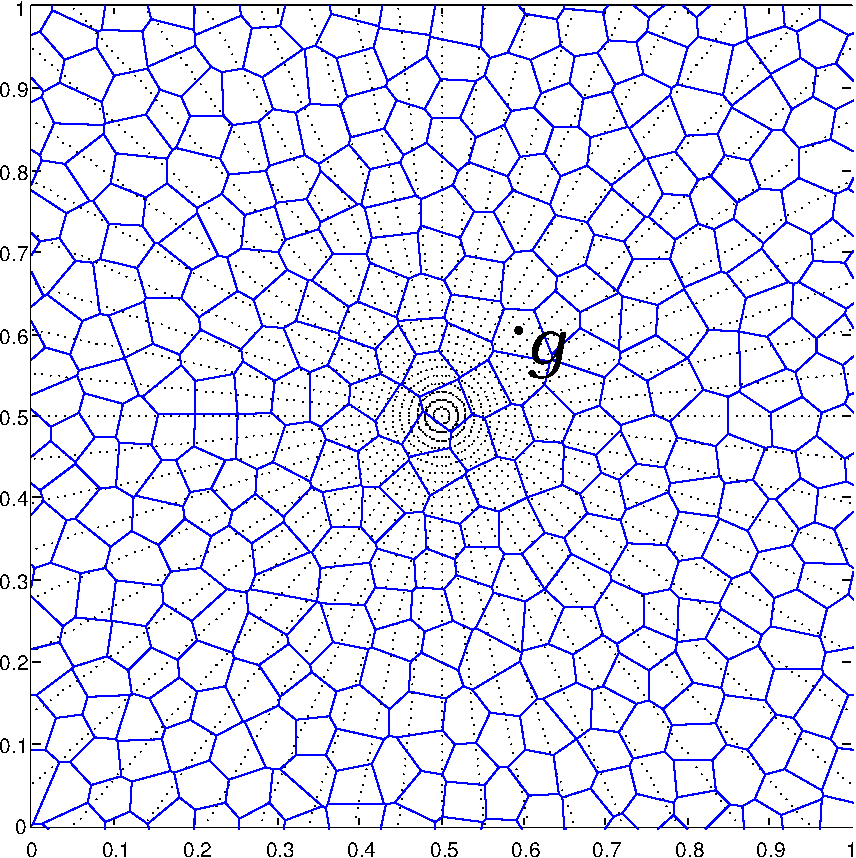
\includegraphics[height=1.2in]{media/voronoi_grid}
}\qquad
\subfigure[Counting neighbors]{
 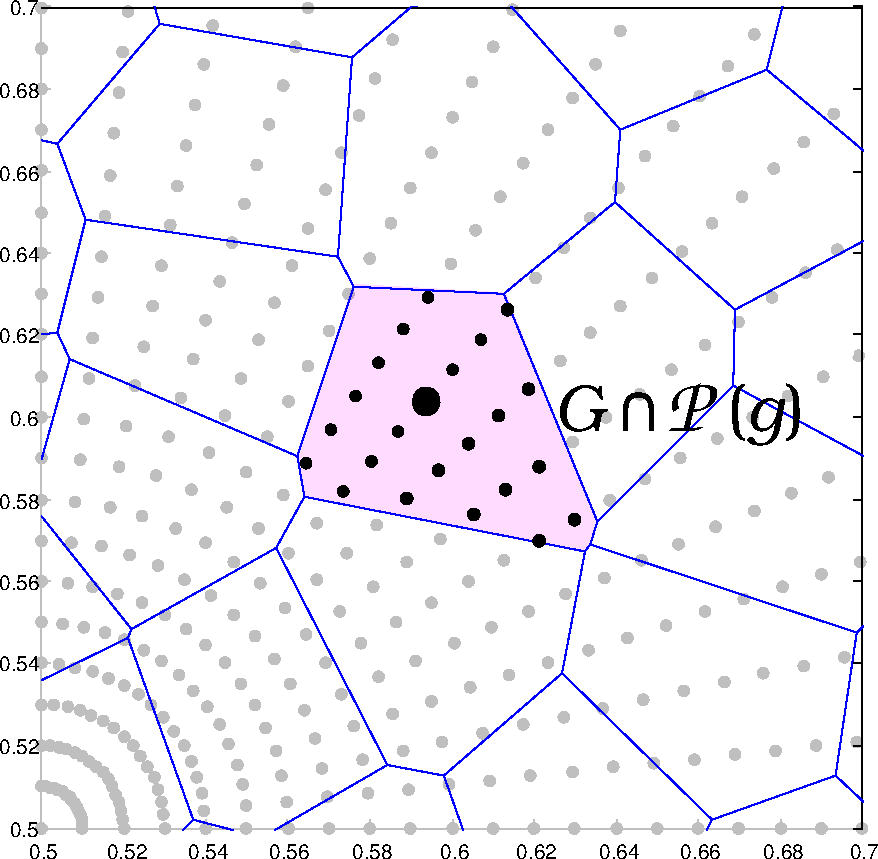
\includegraphics[height=1.2in]{media/voronoi_grid_closeup}
}\qquad
\subfigure[Weight Profile]{
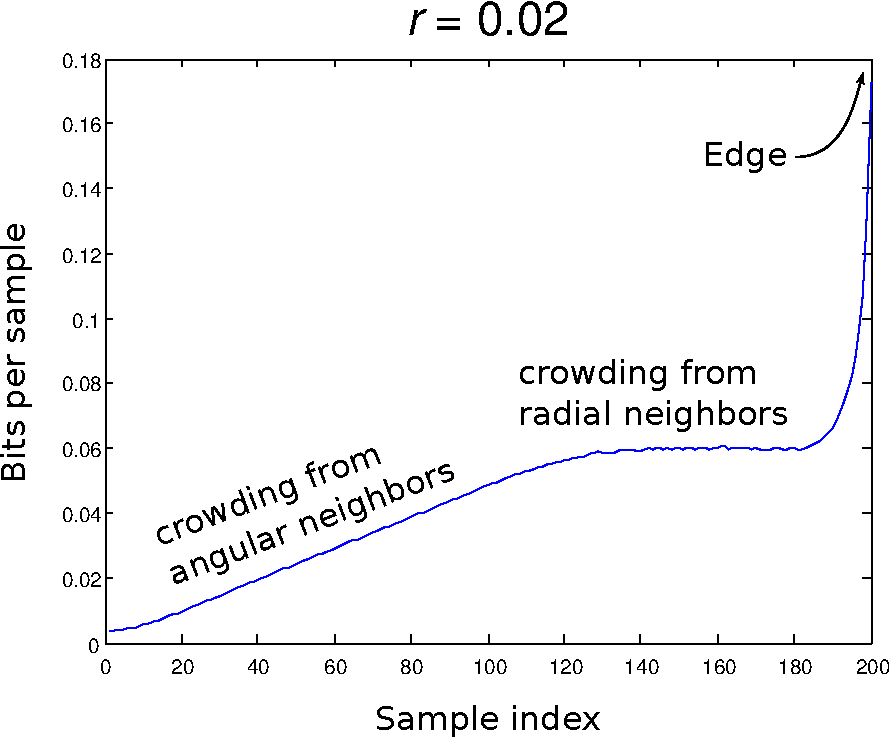
\includegraphics[height=1.2in]{media/weight_profile}
}
\caption{\emph{Computing Sample Weights for a Radial Sampling Grid}\label{fig:weights}
\textbf{(a)} The weight $w_{ij}$ is the expected energy gain from a sample at position $x+g_{ij}$ in $G(x)$.
\textbf{(b)} The entropy of a sample from 
a random coloring of a random partition is taken as the expected value of the reciprocal of the number of samples with which it shares a cell
(argument detailed in \ref{compute_weights}).
\textbf{(c)}  Since the sampling pattern $G$ is radially symmetric, the weights $w_{ij}$ can be described by a radial ``profile''.
The weight profile can be divided into three phases: The first phase, when nodes are likely to share cells with 
angular neighbors, shows a increase in weight as radius increases and radial neighbors get further and further away.
The second phase, when angular neighbors are too far away to share cells, has constant weight.  The third phase, as
we reach the edge of the sampling pattern, shows a rapid doubling of weight, as nodes with many inner and outer 
(smaller or greater radius) neighbors give way 
to nodes with few or no outer neighbors.
}
\end{figure*}


\subsection{Ising-Type Obstacles}
A good obstacle model should incorporate assumptions about the shape, density and grouping behavior of obstacles.  We have considered the obvious strategy of generating several hypothetical completions of partially revealed scenes, then averaging these completed scenes pointwise.
\subsubsection{The Ising Model}
\begin{figure}
\centering
\begin{tabular}{cc}
\begin{tabular}{c}
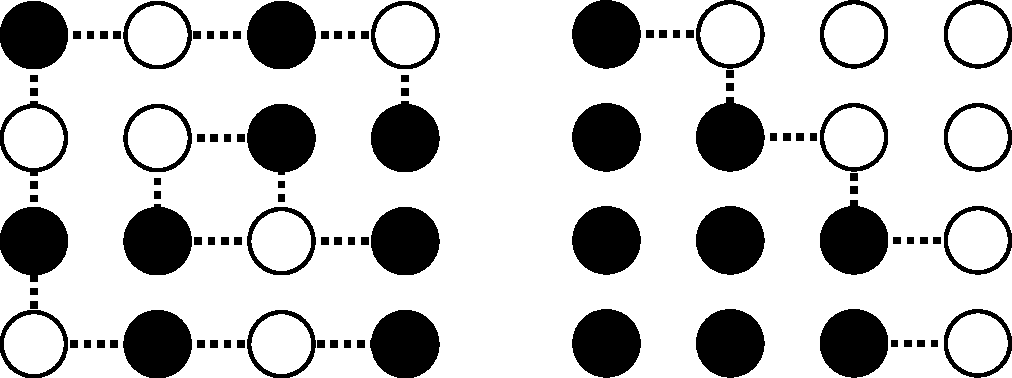
\includegraphics[height=.8in]{hilo_ising}\\
\subfigure[High / Low Energy Configurations]{
\hphantom{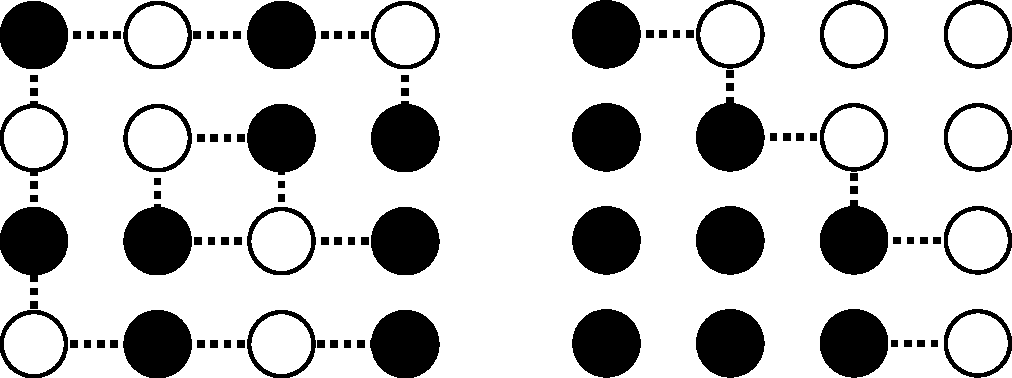
\includegraphics[height=.8in]{hilo_ising}}}
\end{tabular}&
\begin{tabular}{c}
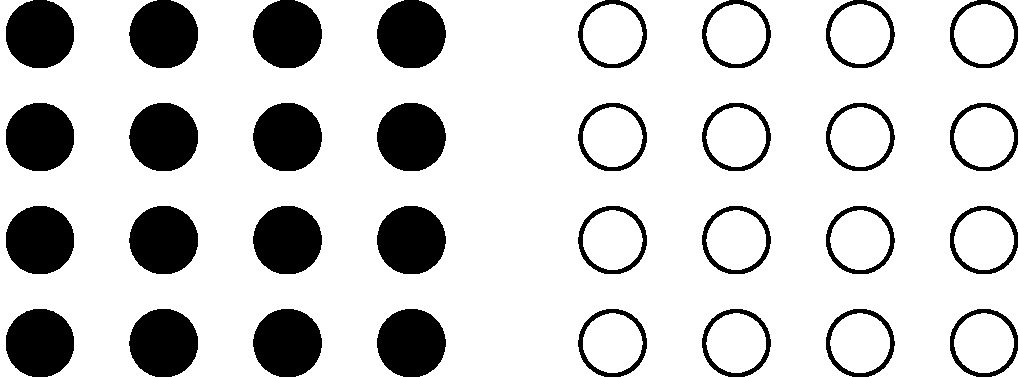
\includegraphics[height=.8in]{min_ising}\\
\subfigure[Minimum Energy Configurations]{
\hphantom{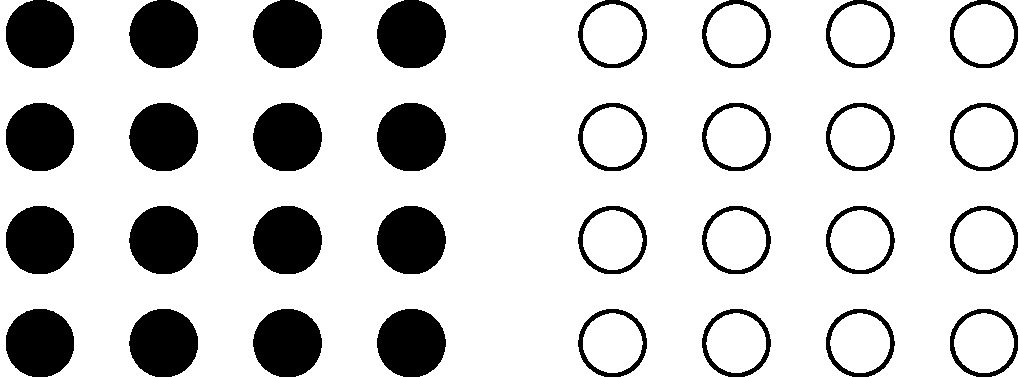
\includegraphics[height=.8in]{min_ising}}}
\end{tabular}
\end{tabular}
\caption{\emph{Ising Model on a $4\times4$ Lattice}
Likelihood under the Ising Model decreases exponentially with the number
of edges between disagreeing nodes.  
Samples from the Ising Model are concentrated near the two minimum energy configurations:
all-white or all-black.
\label{figure: ising}
}
\end{figure}

We will define the Ising Model as 
a probability distribution $\I_{\D}$ on the set of 
binary, $\{-1,1\}$-valued images
$\bigl\{I:\D\to\{-1,1\}\bigr\}$,
where $\D$ is
a 2- (or 3-) dimensional, 4- (or 6-) connected lattice $\D$ (as shown in Fig.\ \ref{fig: ising}).

\begin{equation}
P(I) \propto \exp\bigl(\beta (I_{ij}I_{i+1,j} + I_{ij}I_{i,j+1} + I_{ij}I_{i-1,j} + I_{ij}I_{i,j-1})  \bigr)
\end{equation}

\subsubsection{Sampling from the Ising Model\label{section: monte carlo}}
To generate obstacle hypotheses, we run a Gibbs-sampling implementation 
of the subcritical Ising model (as discussed in \cite{geyer91}), initialized with known obstacles,
and halted after $m$ iterations:
\begin{gather}
\PP_t(I_{ij}^{m+1}=1) = 
\begin{cases}
\frac{\exp(-\beta(H_{ij}^m - 2))}{\exp(-\beta(H_{ij}^m - 2)) + \exp(-\beta(H_{ij}^m - 2))} & x_{ij}\in\U^t\\
1 & x_{ij}\in\A^t\\
0 & x_{ij}\in\O^t
\end{cases}
\end{gather}
with $H^m_{ij} := I^m_{i+1,j} + I_{ij}I_{i,j+1} + I_{ij}I_{i-1,j} + I_{ij}I_{i,j-1}$, and
$\PP_t(I^0_{ij}=1)=0.5$ independently.

This defines a distribution $\I^m_{\D}$ on the set $\bigl\{I^m:\D\to\{0,1\}\bigr\}$. 
Samples and statistics of this family of distributions are shown in Fig.\ \ref{fig: ising}
\begin{figure}
\begin{tabular}{ccccc}
&
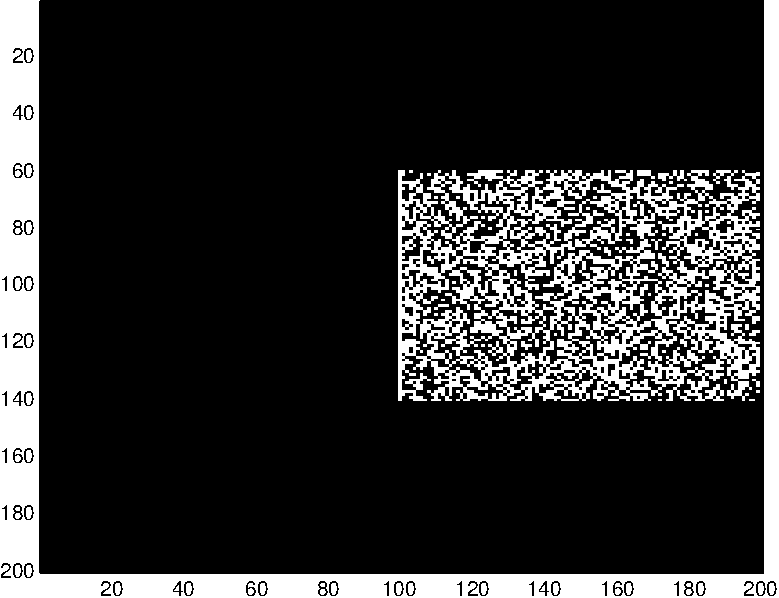
\includegraphics[width=.75in, trim={2.1in .8in .1in .7in}, clip]{ising000}&
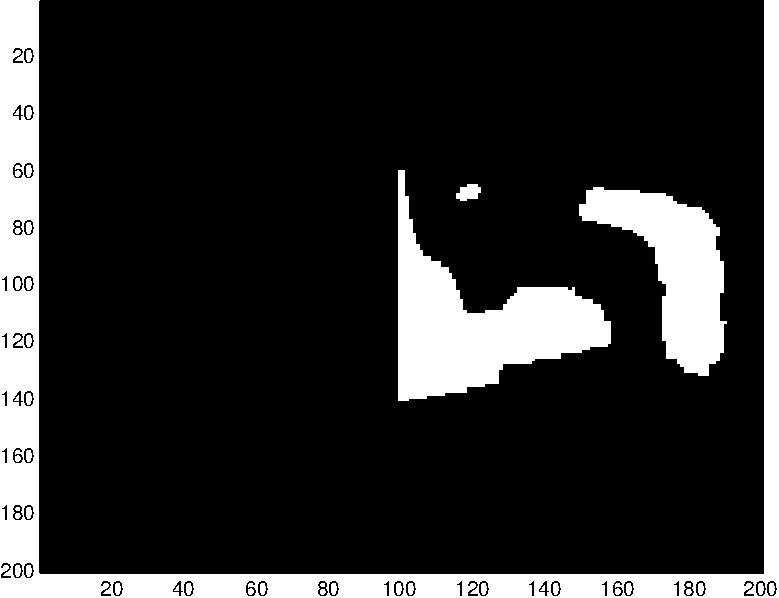
\includegraphics[width=.75in, trim={2.1in .8in .1in .7in}, clip]{ising100}&
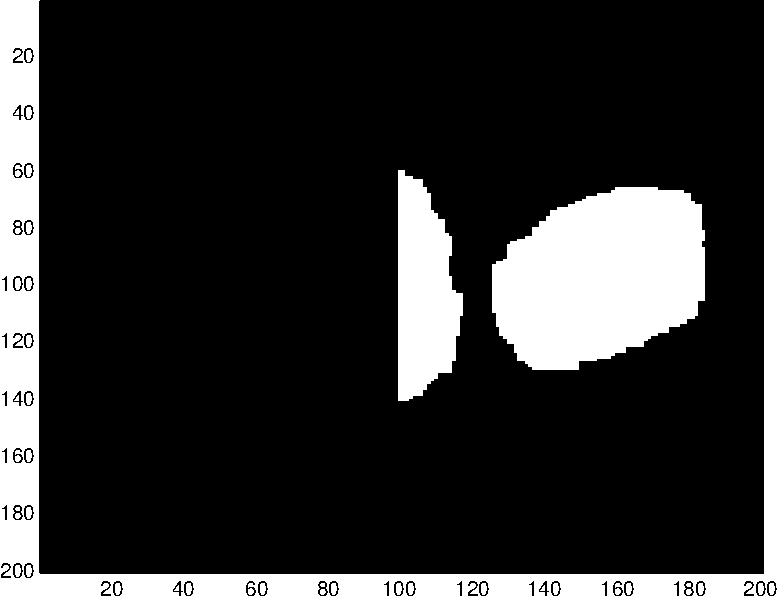
\includegraphics[width=.75in, trim={2.1in .8in .1in .7in}, clip]{ising225}&
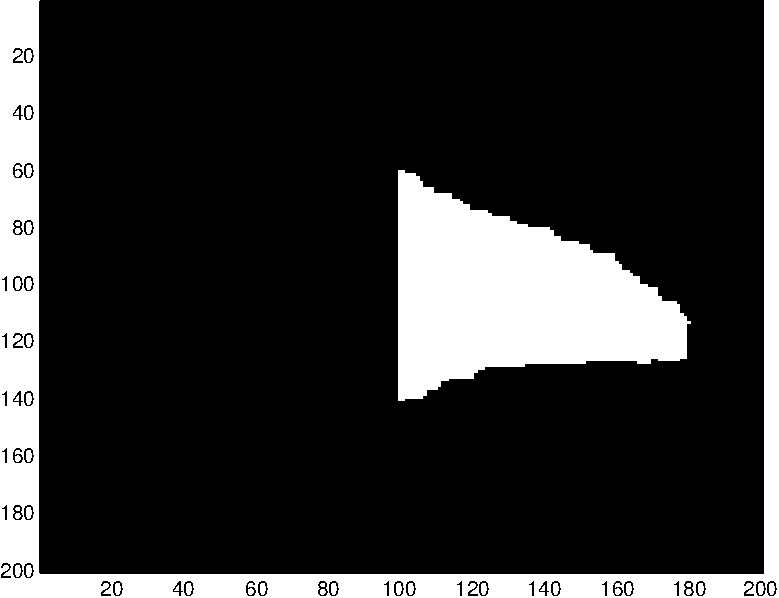
\includegraphics[width=.75in, trim={2.1in .8in .1in .7in}, clip]{ising400}\\
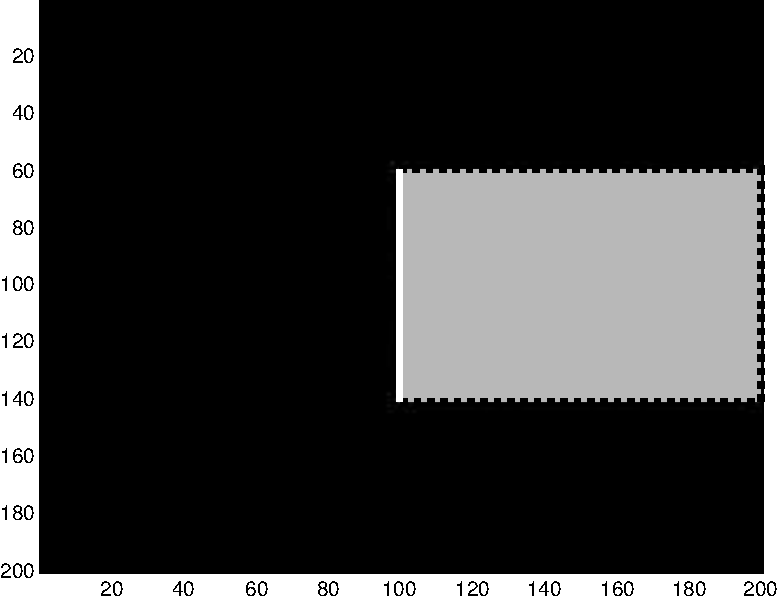
\includegraphics[width=.75in, trim={2.1in .8in .1in .7in}, clip]{visibility}&
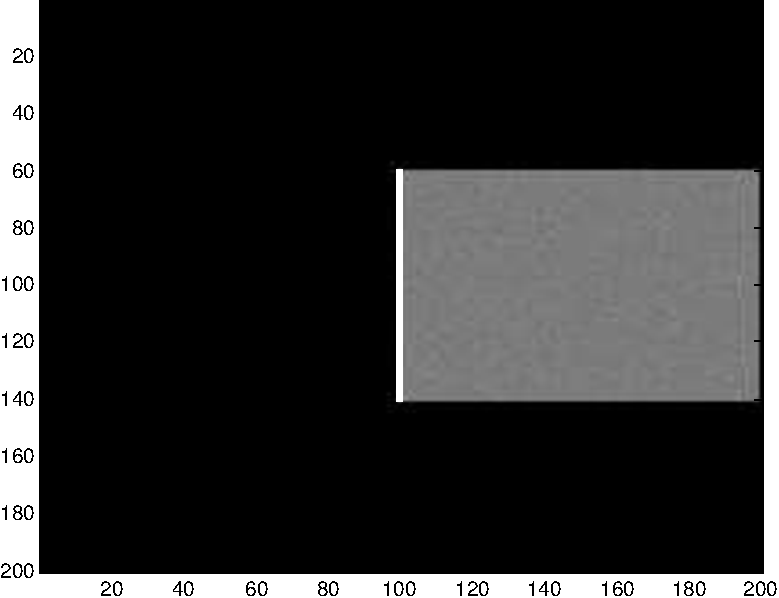
\includegraphics[width=.75in, trim={2.1in .8in .1in .7in}, clip]{marg000}&
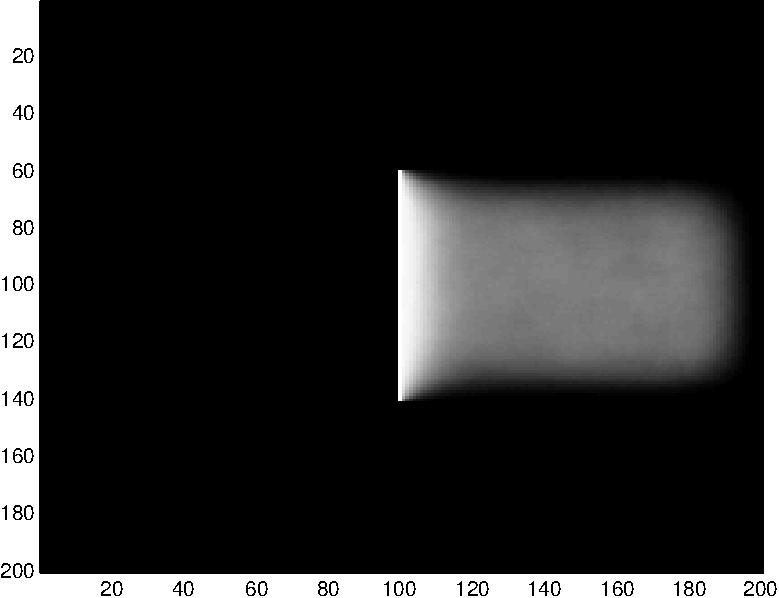
\includegraphics[width=.75in, trim={2.1in .8in .1in .7in}, clip]{marg100}&
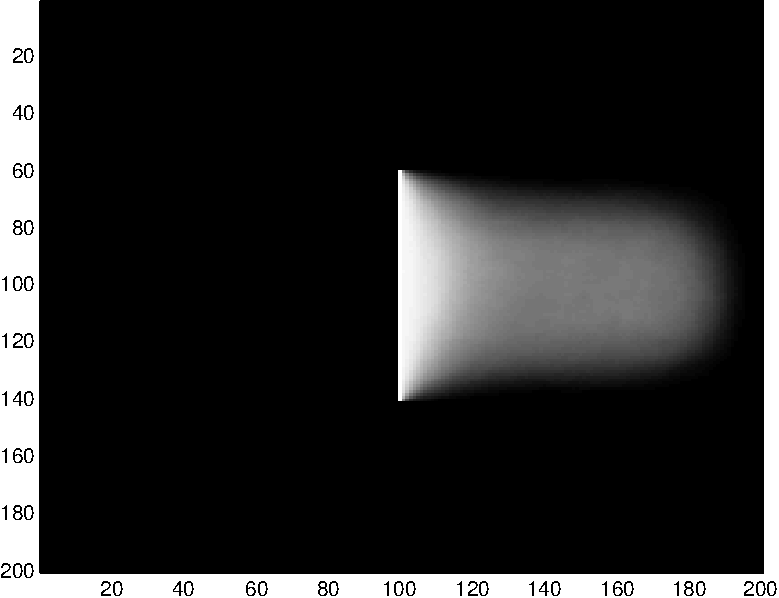
\includegraphics[width=.75in, trim={2.1in .8in .1in .7in}, clip]{marg225}&
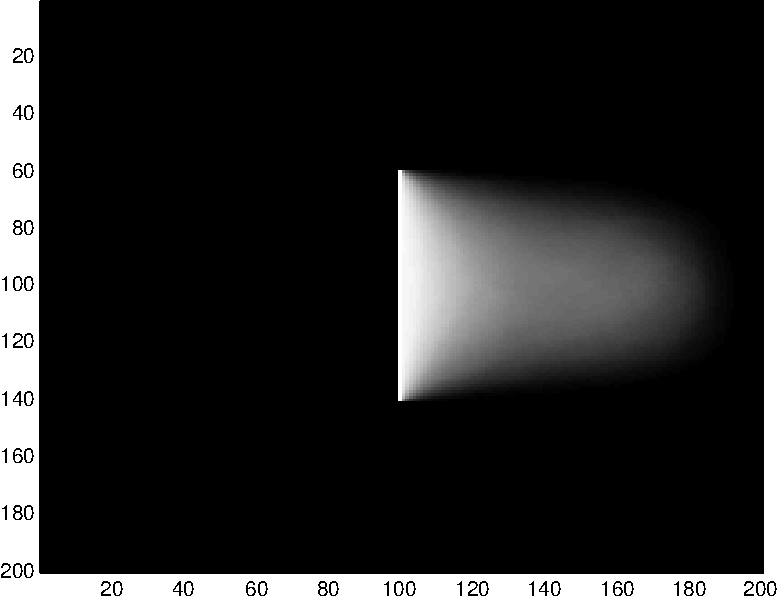
\includegraphics[width=.75in, trim={2.1in .8in .1in .7in}, clip]{marg400}\\
\subfigure[\scriptsize{Visibility}]{
\hphantom{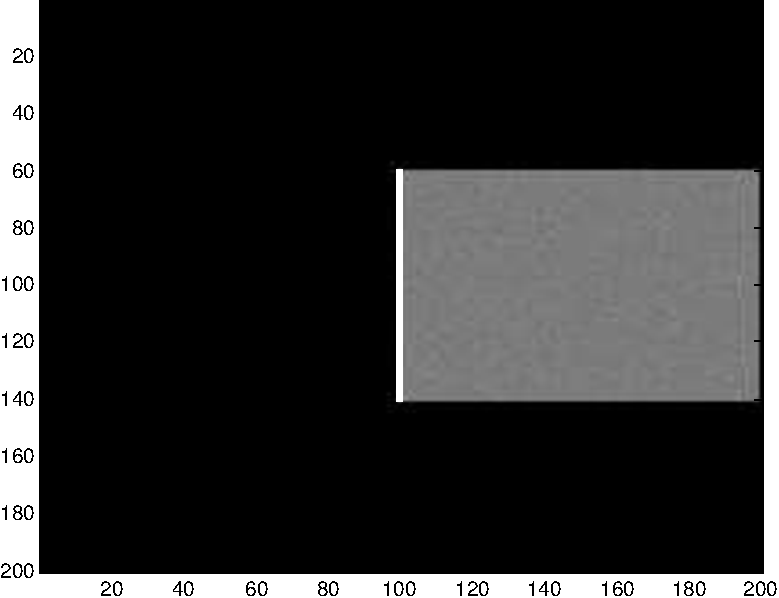
\includegraphics[width=.75in, trim={2.1in .8in .1in .7in}, clip]{marg000}}}&
\subfigure[\scriptsize{0 Iterations}]{
\hphantom{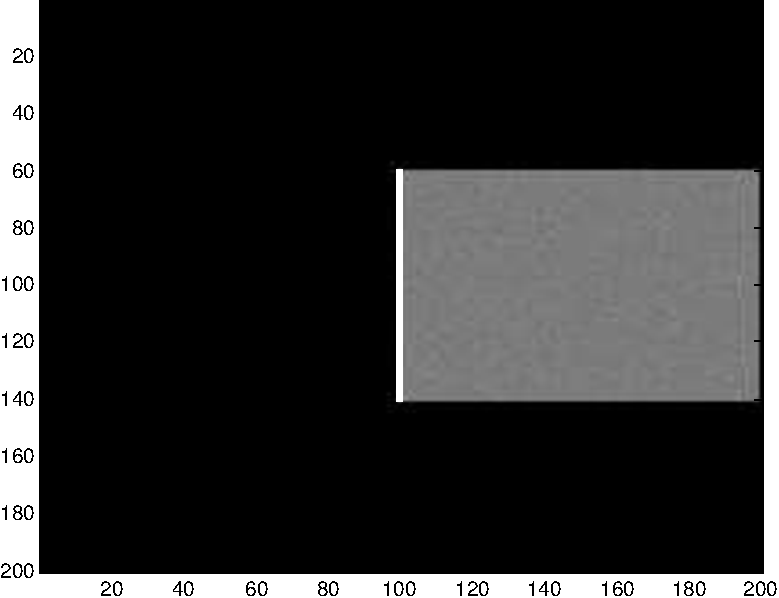
\includegraphics[width=.75in, trim={2.1in .8in .1in .7in}, clip]{marg000}}}&
\subfigure[\scriptsize{100 Iter.}]{
\hphantom{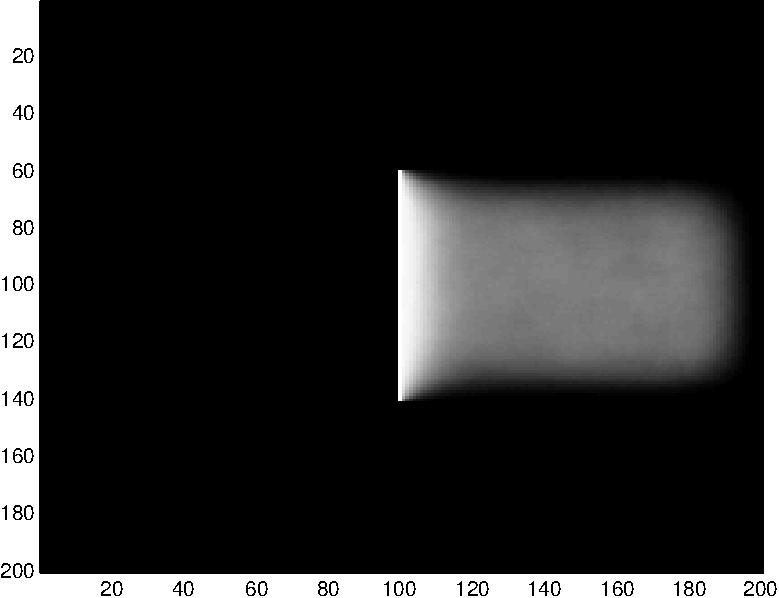
\includegraphics[width=.75in, trim={2.1in .8in .1in .7in}, clip]{marg100}}}&
\subfigure[\scriptsize{200 Iter.}]{
\hphantom{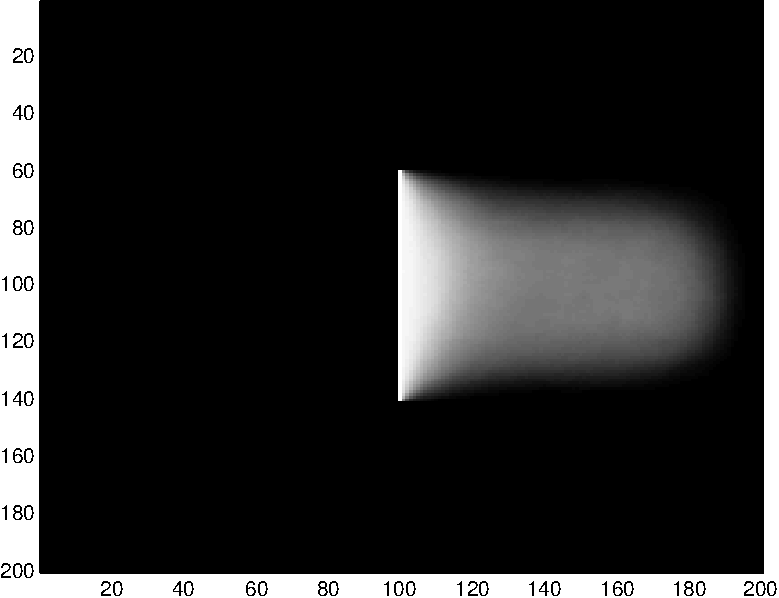
\includegraphics[width=.75in, trim={2.1in .8in .1in .7in}, clip]{marg225}}}&
\subfigure[\scriptsize{400 Iter.}]{
\hphantom{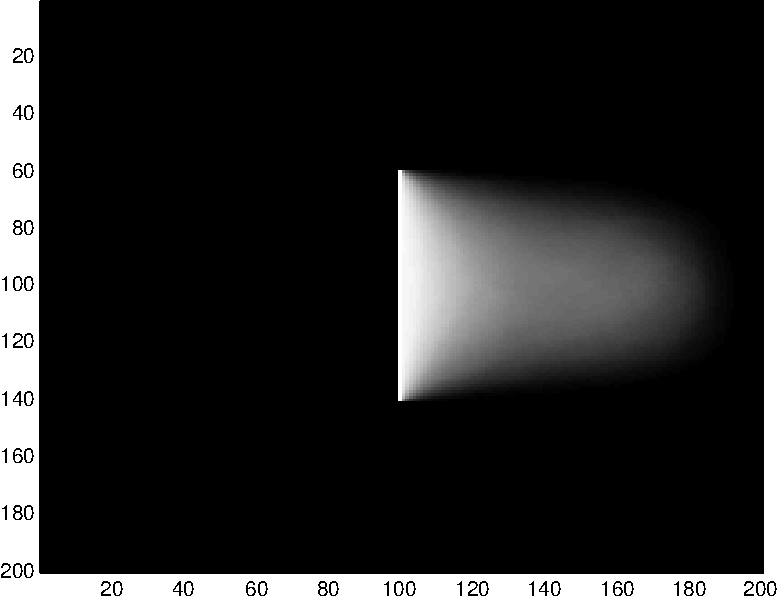
\includegraphics[width=.75in, trim={2.1in .8in .1in .7in}, clip]{marg400}}}
\end{tabular}
\label{fig: ising}
\caption{\emph{Ising-type Obstacle Posterior} (a) The random process described in \ref{section: monte carlo}
is run on a scene with a rectangular shadow region (gray) produced by a
flat obstacle edge (white). Black denotes known free space.
(b)-(e) Top row: Images produced by the process. Bottom row: Average of 1000 runs.
}
\end{figure}

A good choice of the scale parameter $m$ produces
obstacles which ``look like'' (have similar thickness
and curvature to) obstacles that the explorer is likely to see.
The parameter can be estimated by estimating mean free path in the real environment
(e.g. by taking the average of the initial omni-directional range measurement)
and choosing $m$ to match.  Figure \ref{fig: MFP} details how this is done.

Since these scenes are generated using a fixed coloring probability of 0.5,
we normalize the MFP parameter so that $\PP_t(y\in\A)$ can vary:
$$
\PP_t\bigl[\Y_G(x)_{ij}=0 \;|\; \Y_G(x)_{i-1,j}=1\big] \approx
\exp\Biggl(\underset{\mathrlap{\text{line}(x+g_{i-1,j},\,x+g_{ij})}}{\int}\; 
\frac{\log\bigl(\PP_t(y\in\A)\bigr)}{\log(0.5)\,\operatorname{MFP_{0.5}}}\,dy\Biggr)
$$


\begin{figure}
\centering
\begin{tabular}{cccc}
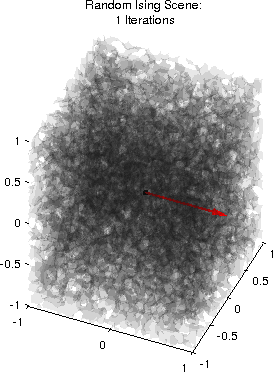
\includegraphics[height=1.2in]{Penetration/ising_cell_001.png} &&
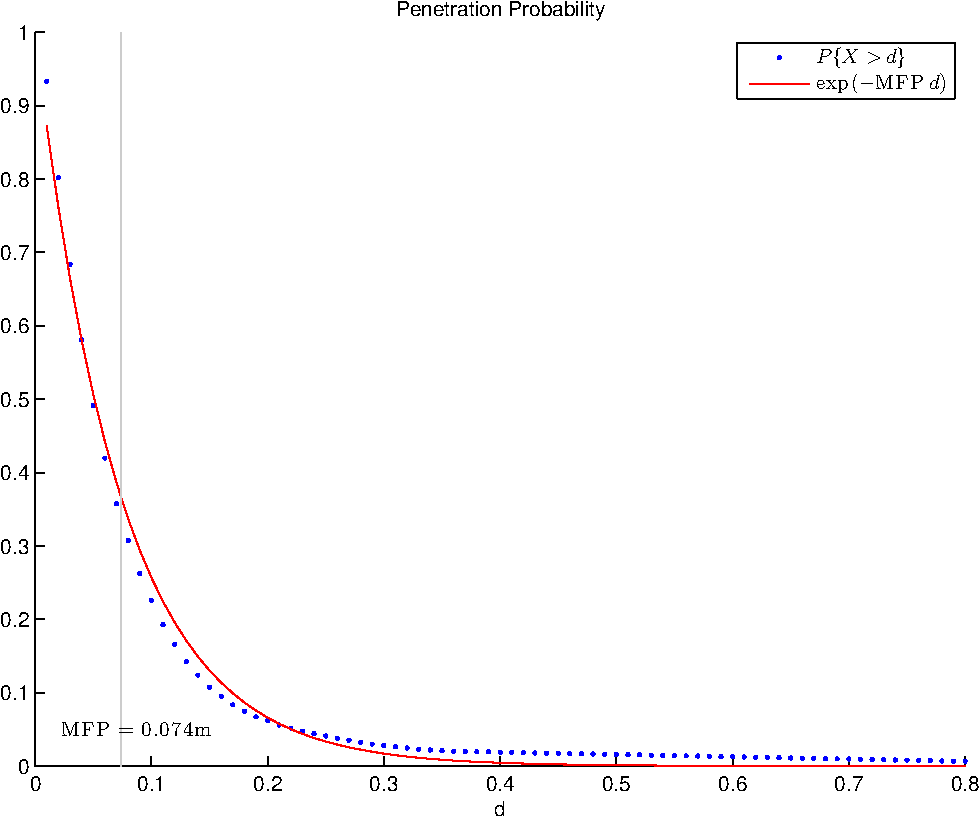
\includegraphics[height=1.2in]{Penetration/ising_penetration_001} &
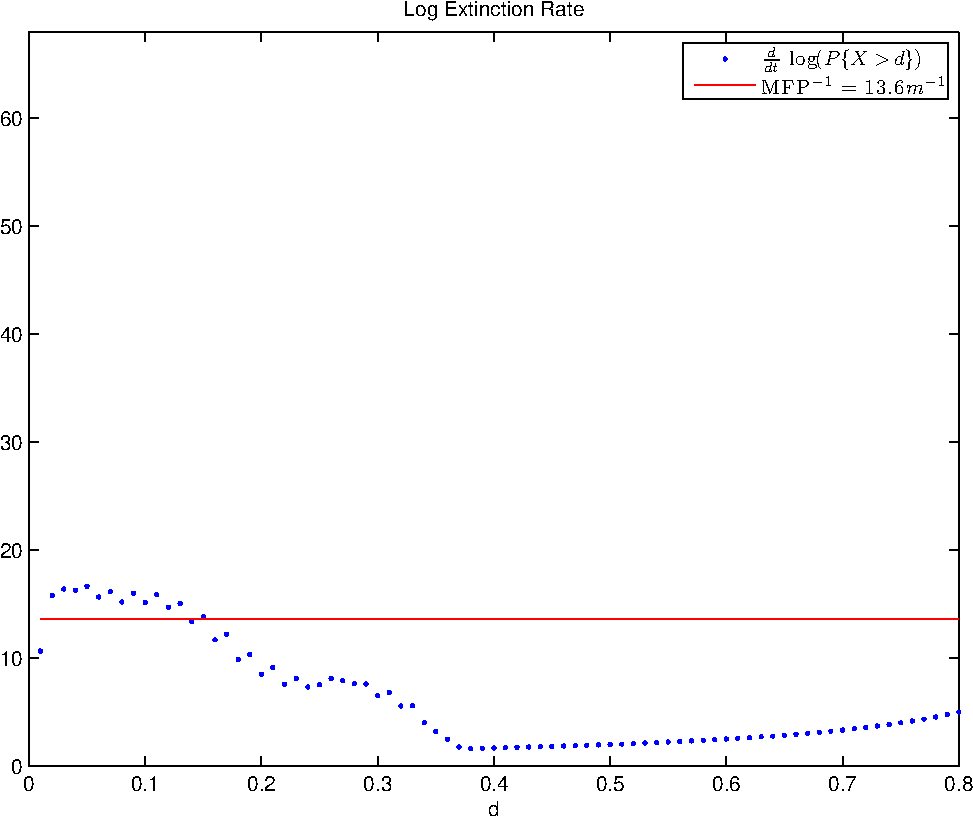
\includegraphics[height=1.2in]{Penetration/ising_extinction_001}\\
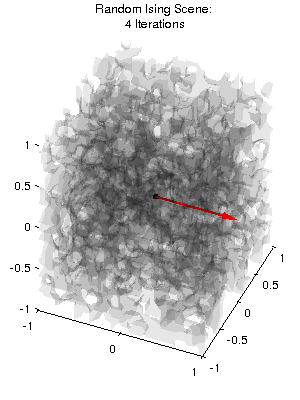
\includegraphics[height=1.2in]{Penetration/ising_cell_004.png} &&
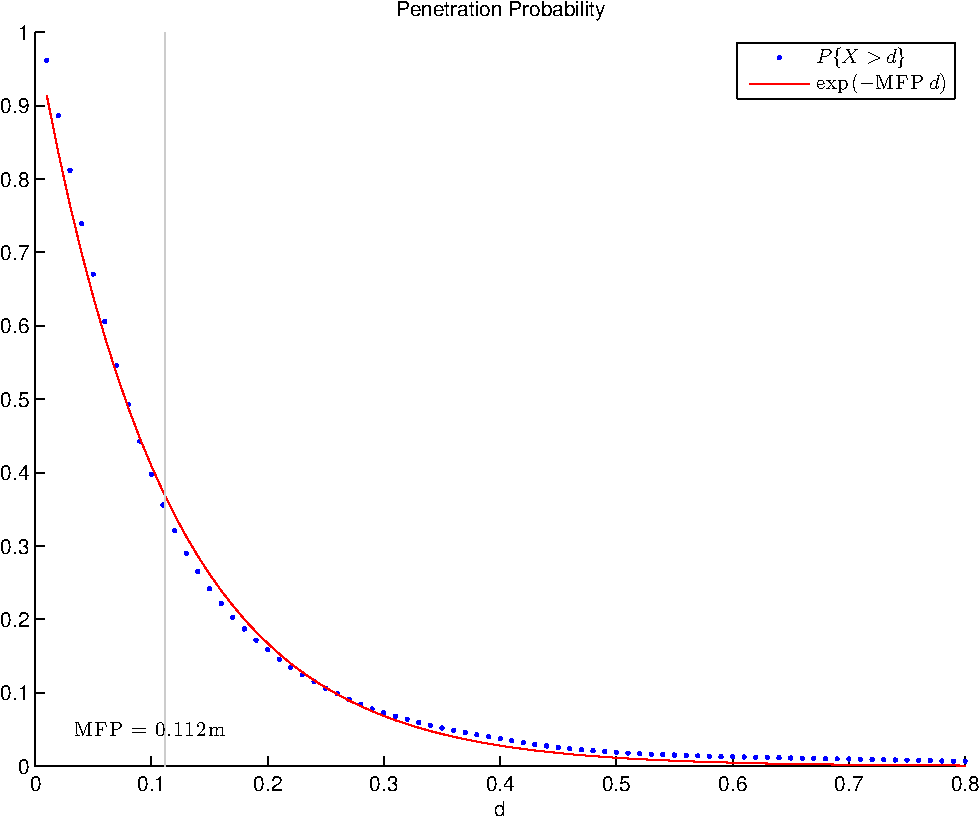
\includegraphics[height=1.2in]{Penetration/ising_penetration_004} &
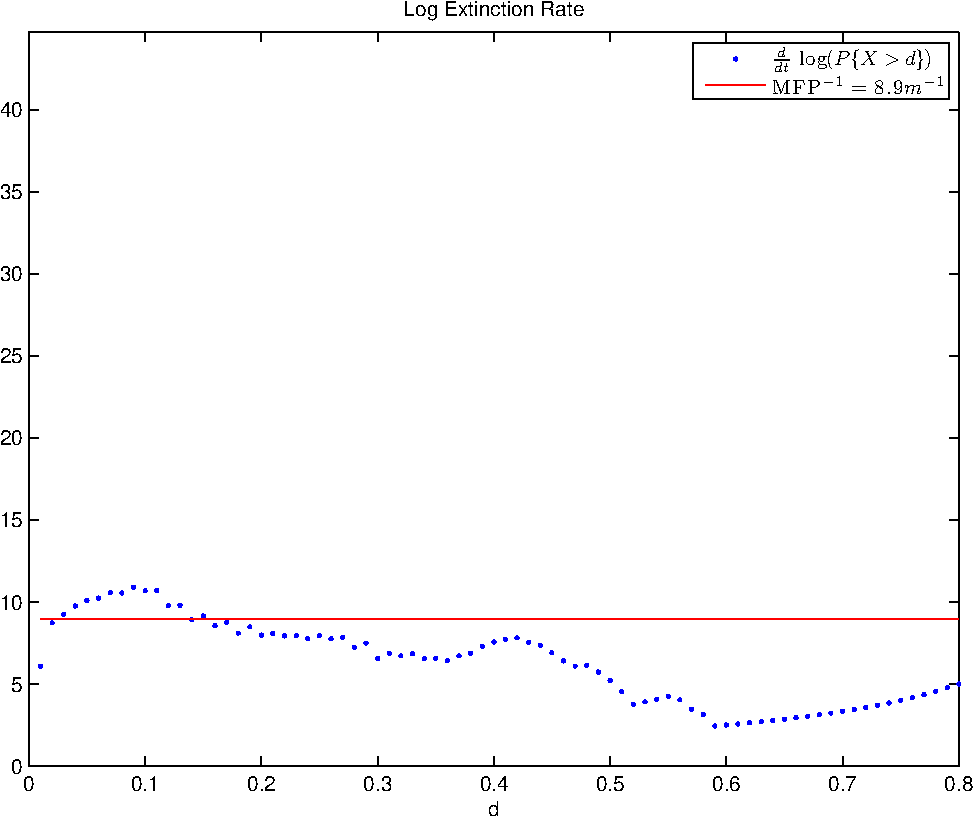
\includegraphics[height=1.2in]{Penetration/ising_extinction_004}\\
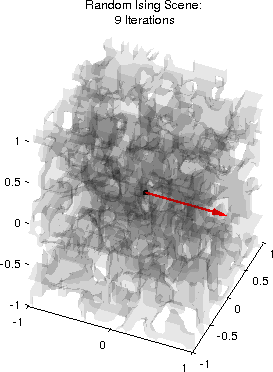
\includegraphics[height=1.2in]{Penetration/ising_cell_009.png} &&
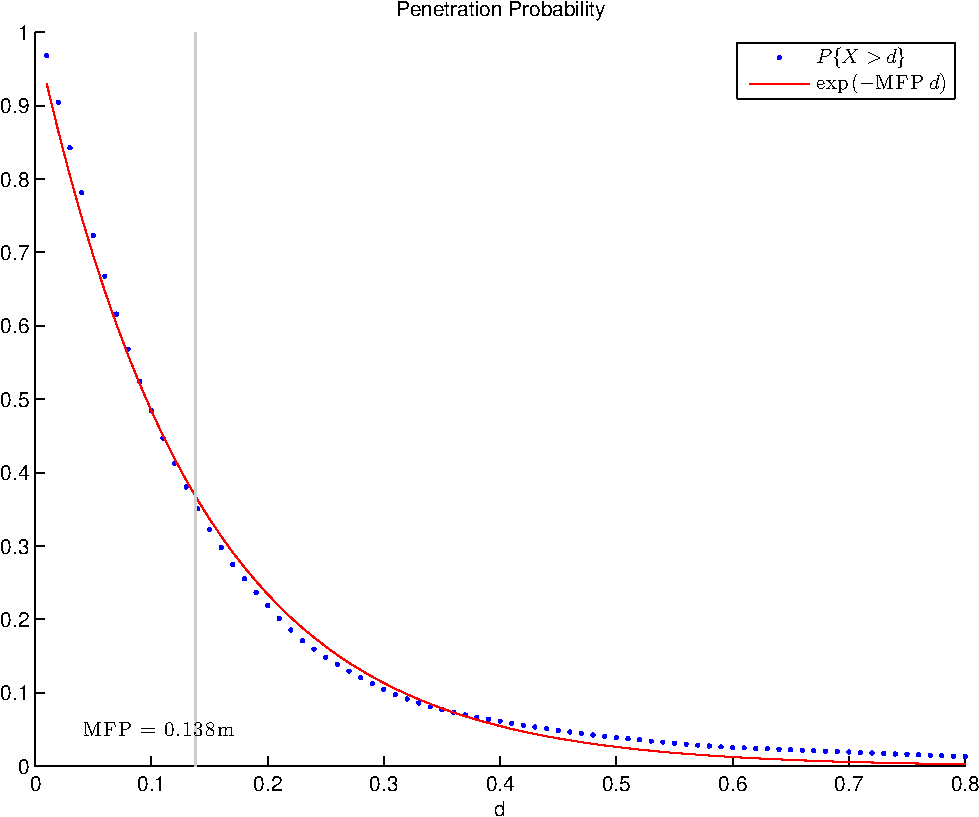
\includegraphics[height=1.2in]{Penetration/ising_penetration_009} &
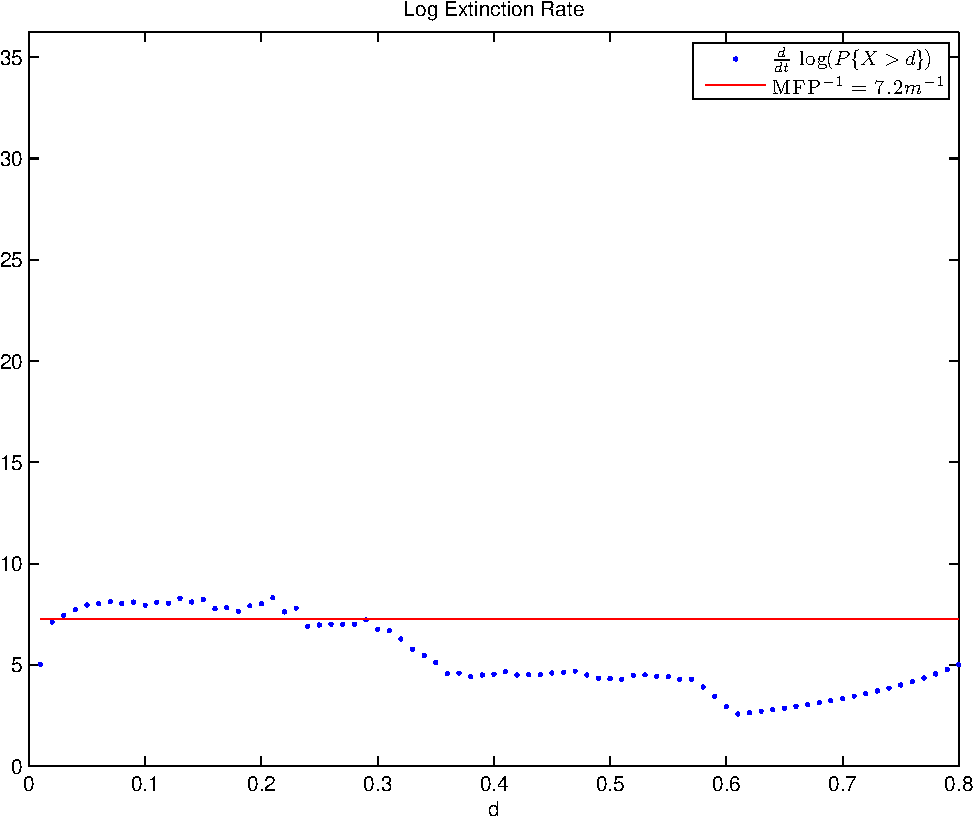
\includegraphics[height=1.2in]{Penetration/ising_extinction_009}\\
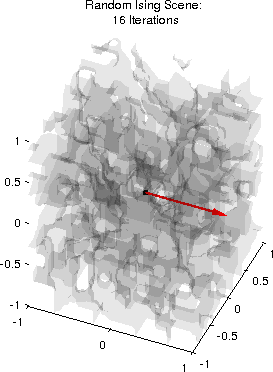
\includegraphics[height=1.2in]{Penetration/ising_cell_016.png} &&
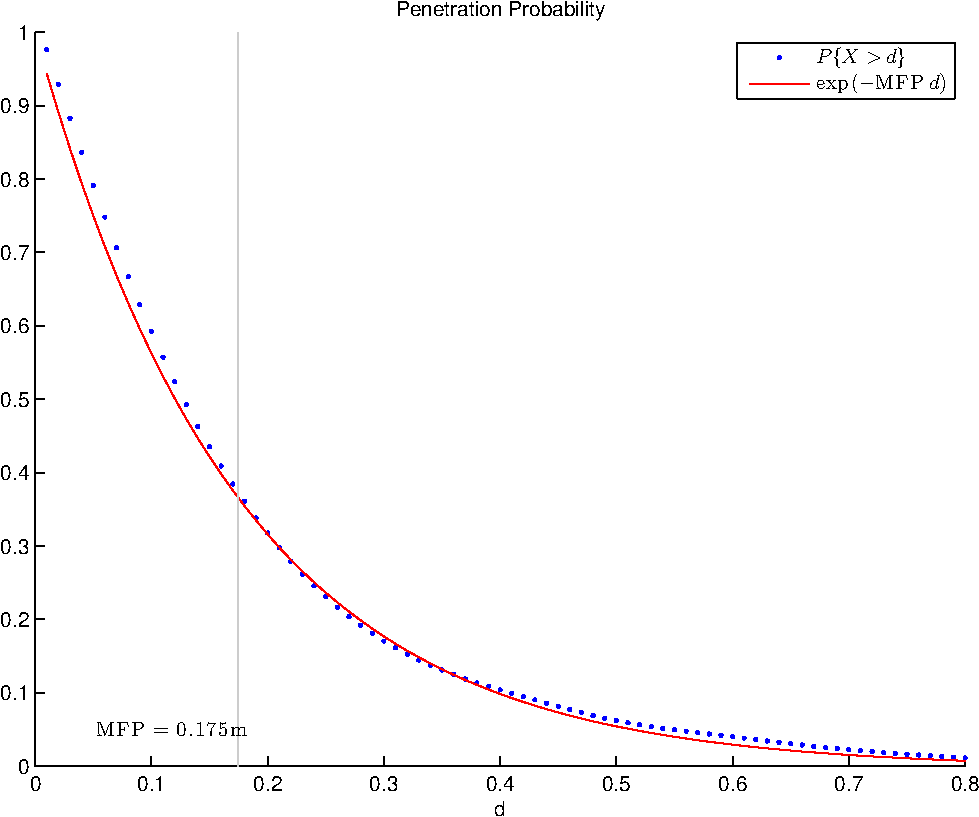
\includegraphics[height=1.2in]{Penetration/ising_penetration_016} &
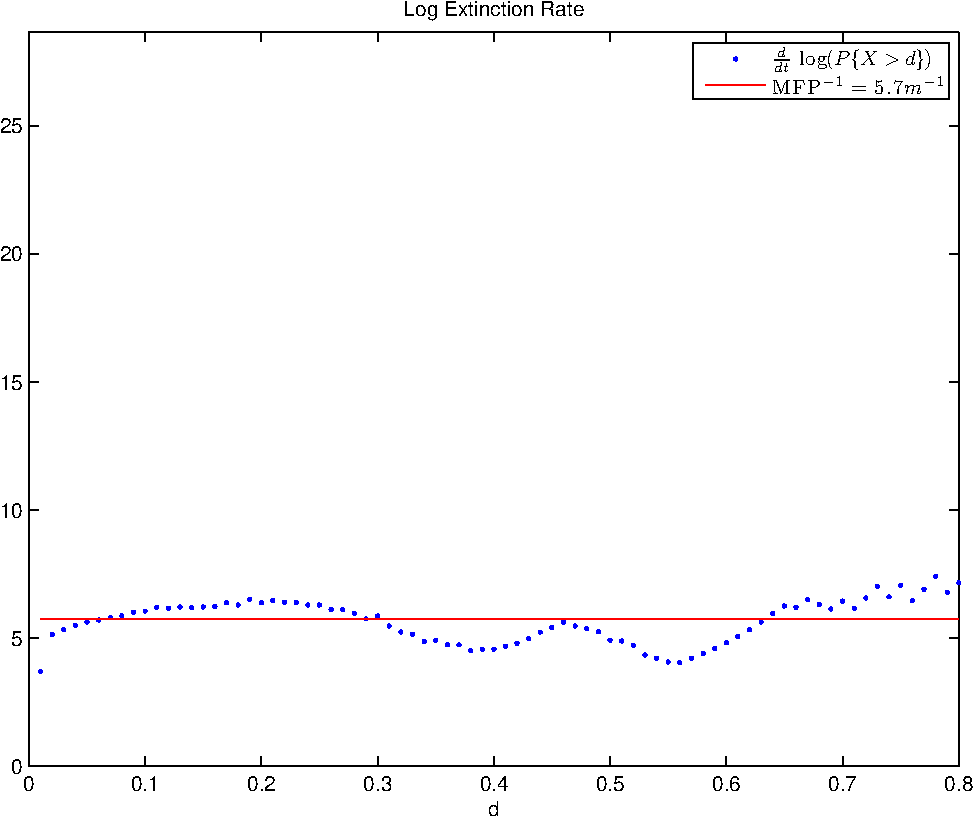
\includegraphics[height=1.2in]{Penetration/ising_extinction_016}\\
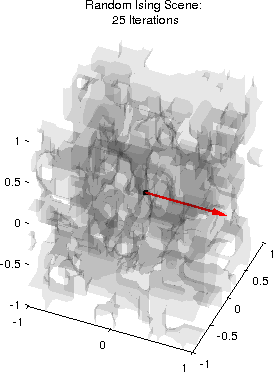
\includegraphics[height=1.2in]{Penetration/ising_cell_025.png} &&
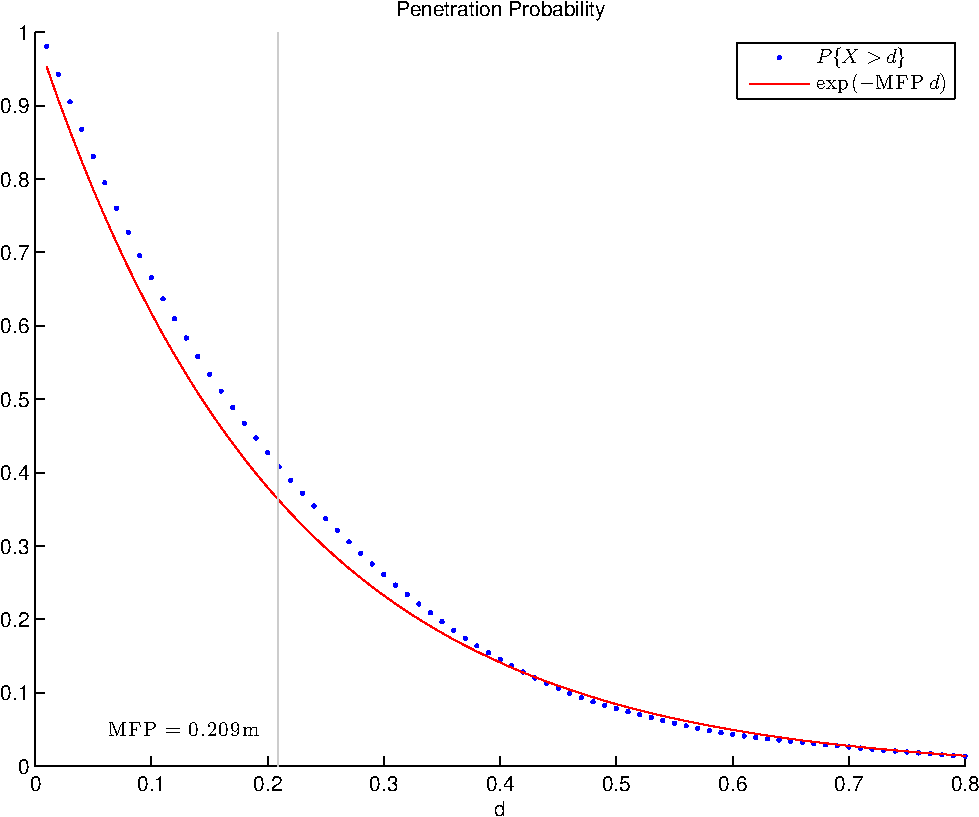
\includegraphics[height=1.2in]{Penetration/ising_penetration_025} &
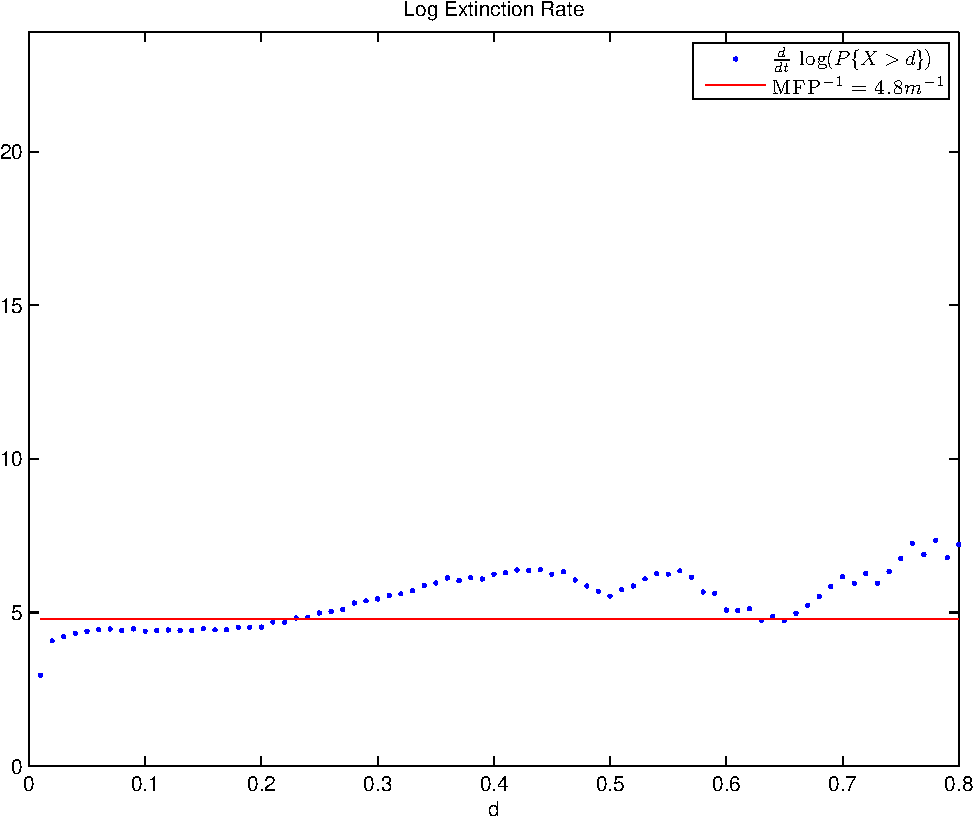
\includegraphics[height=1.2in]{Penetration/ising_extinction_025}
\end{tabular}
\caption{\emph{Extinction Profiles} \label{fig: MFP}
Here we show extinction profiles for Ising scenes with various granularities, indexed by number of update iterations.
Instantaneous mean free path (derivative of log survival probability) and best-fit MFP are plotted together,
showing that extinction in these scenes is well-modeled by an exponential decay.
}
\end{figure}

\subsubsection{Poisson-Disk Approximation}

In order to express the viewpoint quality in
Ising-type in a simple form like (\ref{eq: cell value}),
we make use of
certain statistical properties
shared between our Ising-model scenes 
and randomly-colored partitions of uniformly-sized Voronoi cells.
A Poisson-disc cover $\P^r\subs[-1,1]^2$ is a uniformly
random sampling of points in $[-1,1]^2$ such that 
no two points have distance less than $r$, and no
new point can be added without violating this property.
These sample points induce a Voronoi partition $\L^r=\L(\P^r)$ of $\Omega$.
Random colorings $\xi$ of these Voronoi partitions produce scenes $I^r$
which bear a superficial resemblance to those produced by the Ising
process, as seen in Figure \ref{fig:random coloring}

\begin{figure*}[ht]
\centering
\subfigure[Poisson-Disk Sampling]{
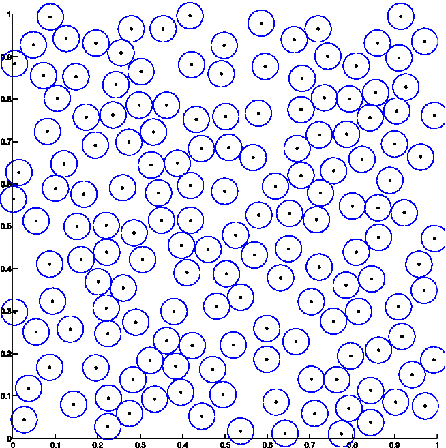
\includegraphics[height=1.3in]{media/poisson_disk}
}
\quad
\subfigure[Voronoi Partition]{
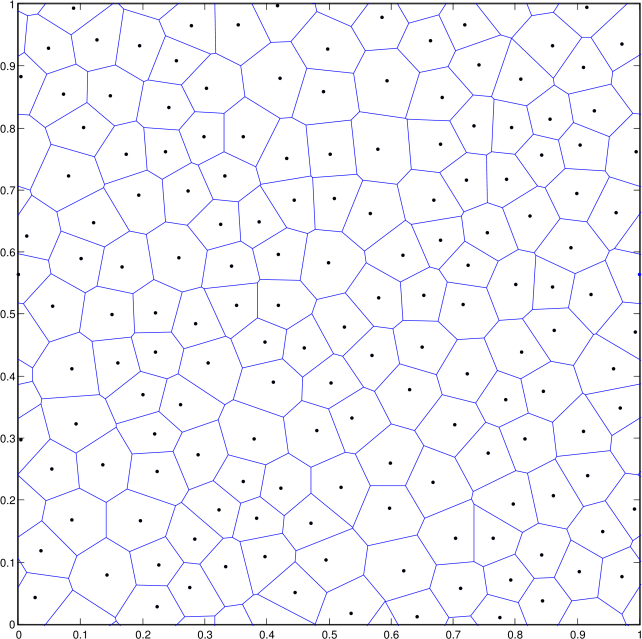
\includegraphics[height=1.3in]{media/voronoi}
}
\quad
\subfigure[Checkerboard]{
\includegraphics[height=1.3in]{media/voronoi_chex}
}
\caption{\emph{Generating Poisson-Voronoi Checkerboard} \label{fig:random coloring}
(a) To produce a scene of desired granulation, we first produce a 
Poisson-Disc sampling of the domain, which gives a maximal set of points
satisfying the property that the distance between two points is no
less than $r$, a granularity parameter. (2)  We compute a Voronoi
partition of the scene based on that sampling 
(3) We color the cells independently,
denoting them as obstacle or free space, with probability 1/2.
}
\end{figure*}

We have found that the Poisson-Voronoi random checkerboard
is a useful surrogate for entropy computations 
involving Ising priors.
For a given set of points $\{x_k\}\subs\Omega$,
the entropy $\HH[ I^m(\{x_k\})]$ 
of sampling a random Ising scene $ I^m$, with scale parameter $m$,
can be estimated from the entropy $\HH[ IPV^r(\{x_k\})]$,
for a random Poisson-Voronoi checkerboard.
We have found a strong empirical correspondence between
these joint entropies, for sampling sets of ten or fewer
(estimating the distribution of the boolean random variable $ I^m(\{x\})$,
for a \emph{single} sampling set $\{x\}\subs\Omega$
requires on the order of $2^{|\{x\}|}$ random Ising scenes - 
as we will see, it is much less taxing to generate the Poisson-Voronoi checkerboards).
Correlations between these entropies, for a range of values of $m$
and $r$, are plotted in Figure \ref{fig:comparisons}.
Good matches are highlighted in pink.


\begin{figure*}[h]
\centering
\subfigure[Ising Textures]{
\includegraphics[height=.85in]{media/entropy_ising}
}
\\
\subfigure[Corresponding Voronoi Checkerboards]{
\includegraphics[height=.85in]{media/entropy_chex}}
\caption{\emph{Poisson-Voronoi Checkerboard}\label{fig:Correspondence}
There is a superficial resemblance Ising-type obstacles 
and Voronoi checkerboards with appropriate scale parameters.
}
\end{figure*}

\subsubsection{Computing the Weights $w_g$ \label{compute_weights}}
The statistical correspondence between Ising scenes and Voronoi checkerboards 
allows for the efficient computation of weights $w_i$.
The joint entropy of samples from the random checkerboards is
easily expressed as a weighted sum of the marginal entropies of the samples.

Recall that we can define
\begin{equation}
w_i = \EE\left[\frac{1}{\#(G\cap\P^r(g))}\right].
\end{equation}
That is, $G$ is the average of the reciprocal of the number of grid points in $G$ that share a 
Voronoi cell with $g$, as determined by a random Poisson disk sampling (see Figure \ref{fig:random coloring})

These weights can be computed numerically, for a given Poisson disk radius $r$ and sampling pattern $G$,
simply by generating many random Poisson-Voronoi partitions of the region surrounding $G$
and averaging the reciprocal of the number of $g$'s neighbors in $G$.  
If the sampling pattern is radially symmetric, weights only depend on radial index.  Weight profiles for several
Poisson disk radii $r$ are shown in Figure \ref{fig:weights}.

\begin{figure}
\includegraphics[width=5in]{media/weight_profiles}
\caption{\emph{2D Weight Profiles for Various $r$}
Using the counting technique described in \ref{section: indcells}, 
we compute the information contribution, in bits, 
of samples at different (radial) positions on the radial sampling pattern (See Fig.\ \ref{fig: grids}),
with regard to Poisson-Disc Voronoi scenes of various scales.
In this case, we have 30 angular divisions and 200 radial divisions within a maximum radius of one unit.
}
\end{figure}

\begin{figure}
\centering
\subfigure[Pattern]{
\includegraphics[height=.9in]{samples.png}}%\qquad
%\subfigure[Conic Section of Voronoi Cells]{
%\includegraphics[height=1in]{im003.png}}\\
\subfigure[r=0.02]{
\includegraphics[width=.9in]{W02}}
\subfigure[r=0.04]{
\includegraphics[width=.9in]{W04}}
\subfigure[r=0.08]{
\includegraphics[width=.9in]{W06}}
\subfigure[r=0.06]{
\includegraphics[width=.9in]{W08}}
\caption{\emph{3D Weight Profiles for Various $r$}
The counting technique described in \ref{section: indcells} is applied 
to 3D Poisson-Disc Voronoi Scenes, drawing from a spherical sampling pattern (a)
with 30 azimuthal, 200 radial, and 11 elevation divisions.  Again, radial symmetry around the 
vertical axis allows us to ignore azimuthal index.
}
\end{figure}


\begin{figure*}
 \centering
 \includegraphics[scale=0.4]{media/left_combos_hilite} 
 \includegraphics[scale=0.4]{media/right_combos_hilite}
 \caption{\emph{Entropy Comparisons}\label{fig:comparisons}}
\end{figure*}

\iffalse
\subsection{Extensions}

\subsubsection{Sensor Accuracy}

The measure of accuracy that we are interested in
is 


Even if the search domain is infinite, 

Which, for finite time 

Restrict the effective domain of the exploration problem

Here we 

\begin{enumerate}
 \item Error due to imperfect collimation of the laser beam, which
bound the probability of true detection of an obstacle in its line of sight,
a bound which decreases with the square of distance.

\item Error due to miscalibration of the , which can usually be modeled
by a variability in measurments whose magnitude is proportional to
the size of the measurements.

\item Error due to atmospheric anomalies, which can also be 
modeled as a percent-error.

\item Finally, even a perfectly-accurate finite-resolution machine is 
limited by the number of significant figures
in the measurements it produces.
\end{enumerate}

\fi

%\subsubsection{Anisotropic Ising Model}



\section{Exploration}

\iffalse
The exploration problem is formally equivalent with a \emph{partially observed Markov decision process}\break $\langle S, A, \Y, T, \Omega, R \rangle$, where $S$ is a set of states of the environment, which is partially observed due to topological uncertainty introducing obstacles, $A$ is a finite set of actions available from state $S$, which correspond to the transitions to the visible positions in the space, $\Y$ is a set of observations, $T: S \times A \times S \rightarrow [0, 1]$ is a set of transition probabilities (in our case is $1$ for the state $s' \in S$ that corresponds to the best-next view and $0$ for every other state), $\Omega: S \times A \times \Y \rightarrow [0, 1]$ is a set of conditional observation probabilities and $R: S \times A \times S \rightarrow \mathcal{R}$ is the immediate reward received by applying the action $A$ when we are in state $S$.
\fi

Having the range detector measurements (the observations) available $\Y(x_i) \in \Y$ at time $t_i$, we 
estimate $p_t(x)$ for a regular sampling of points in $\A_t$.  Our next waypoint $x_{t+1}$ is selected as
\begin{equation}
 x_{t+1} = \arg\max_{x\in\A} E_t(x)
\end{equation}
Exploration terminates when $E_t(x)$ falls below a certain threshold for all points on the sample grid.
%\section{Implementation}

\begin{figure}
\centering
 \begin{tabular}{ccc}
\includegraphics[width=1.5in]{2D/scene_01}&
\includegraphics[width=1.5in]{2D/marginal_01}&
\includegraphics[width=1.5in]{2D/energy_01}\\
\includegraphics[width=1.5in]{2D/scene_02}&
\includegraphics[width=1.5in]{2D/marginal_02}&
\includegraphics[width=1.5in]{2D/energy_01}\\
\includegraphics[width=1.5in]{2D/scene_03}&
\includegraphics[width=1.5in]{2D/marginal_03}&
\includegraphics[width=1.5in]{2D/energy_03}\\
\includegraphics[width=1.5in]{2D/scene_04}&
\includegraphics[width=1.5in]{2D/marginal_04}&
\includegraphics[width=1.5in]{2D/energy_04}\\
\includegraphics[width=1.5in]{2D/scene_05}&
\includegraphics[width=1.5in]{2D/marginal_05}&
\includegraphics[width=1.5in]{2D/energy_05}\\
\subfigure[Visibility]{
\hphantom{\includegraphics[width=1.5in]{2D/scene_05}}}&
\subfigure[Marginal Likelihood]{
\hphantom{\includegraphics[width=1.5in]{2D/marginal_05}}}&
\subfigure[Viewpoint Quality]{
\hphantom{\includegraphics[width=1.5in]{2D/energy_05}}}\\
\end{tabular}

\end{figure}

\begin{figure}
\begin{tabular}{ccc}
\includegraphics[width=1.5in]{view_01}&
\includegraphics[width=1.5in]{marginal_01}&
\includegraphics[width=1.5in]{energy_01}\\
\includegraphics[width=1.5in]{view_02}&
\includegraphics[width=1.5in]{marginal_02}&
\includegraphics[width=1.5in]{energy_02}\\
\includegraphics[width=1.5in]{view_03}&
\includegraphics[width=1.5in]{marginal_03}&
\includegraphics[width=1.5in]{energy_03}\\
\includegraphics[width=1.5in]{view_04}&
\includegraphics[width=1.5in]{marginal_04}&
\includegraphics[width=1.5in]{energy_04}\\
\includegraphics[width=1.5in]{view_05}&
\includegraphics[width=1.5in]{marginal_05}&
\includegraphics[width=1.5in]{energy_05}\\
\subfigure[Visibility]{
\hphantom{\includegraphics[width=1.5in]{view_05}}}&
\subfigure[Marginal Likelihood]{
\hphantom{\includegraphics[width=1.5in]{marginal_05}}}&
\subfigure[Viewpoint Quality]{
\hphantom{\includegraphics[width=1.5in]{energy_05}}}\\
\end{tabular}
\end{figure}

\subsection{Performance Bounds}

These bounds depend on some conjectured properties of the Ising-model marginal visibility probabilities $p_t(x) = \PP_t[x\in\V]$.  
Assume a fixed scaled-iteration-number $\mu := m/\text{scale(m)}$, and sufficiently-small grid spacings in $G$:

\begin{conj}[Bounded Curvature of $p_t$]
\label{equi}
For any threshold $\epsilon>0$, 
there is a finite constant $K = K(\epsilon)$, independent of $\V_t$ and $\O_t$, such that
(some suitable discrete analogue of) the boundary curvature of the level set $\{x:p_t(x) \leq 1-\epsilon\}$ is bounded above by $K$.
\end{conj}
The result in \cite{lacoin2011zero}, that the zero-temperature Ising model acts (in the scaling limit) as a curve-shortening flow on the level curves of binary images,
suggests that the iterative low-temperature simulations that generate our hypothetical scenes
will produce predictably-rounded hypothetical obstacles.  In turn, it suggests that their pointwise average will have predictably-rounded level curves.

\bigskip
Now, let $\V_t^r$ be the set of points in $\V_t$ that lie at distance $r$ or greater from points in $\O_t$, and let $\V_t^r(x_0)$ be the path-component of $\V_t^r$ containing $x_0$.  Next, we make a sort of equicontinuity assumption:
\begin{conj}
For $p$ sufficiently close to 1, and radius $r>0$, there is a second radius $0<r\1\leq r$, independent of $\V_t$ and $\O_t$,
such that 
\begin{align*}
\bigl(x\in\V_t^r \;\wedge\;&
p_t(x)>p \;\wedge\;
d(x,z)<r\1\bigr)\\
&\qtx{implies that} p_t(z)\geq\tfrac{1}{2}.
%\label{equi}
\end{align*}
\end{conj}
This would guarantee all points sufficiently far from known obstacles, with sufficiently high marginal probability, lie within disks of high marginal probability.  These conjectures, if true, imply the following:

\begin{lemma}
Given a probability threshold $p_{\text{thresh}}>0$, and radius $r$, there is an energy threshold $E_{\text{thresh}}>0$ such that any point $x\in\V_t^r$ with $p_t(x)>p_{\text{thresh}}$ will
induce an energy $E_t(y)>E_{\text{thresh}}$ at a nearby point $y$.
\end{lemma}
\emph{Proof:}
Let $r\1$ be as described in Conjecture \ref{equi}, where $r$ and $p_{\text{thresh}}$ take the place of $r$ and $p$.  Then let
\begin{align*}
E_{\text{thresh}} =  
2^{-\lambda r\1/2}&
\pi \min\left\{K(p_{\text{thresh}})^{-2},\,\tfrac{1}{4}r^{\prime 2}\right\}\\
&\cdot\left(-\log p_{\text{thresh}}\right).%\label{bound}
\end{align*}
Each of the three terms on the RHS is a lower bound of the corresponding term in the energy calculation, centered at $x$.  The first bounds the area of the intersection 
between the level set $\{x:p_t(x)>p_{\text{thresh}}\}$ 
and the disk of radius $r\1$, centered at $x$.
For points $z$ in this region, $\frac{1}{2} \leq p_t(z) \leq p_{\text{thresh}}$, and so
$$2^{-\lambda r\1/2}\leq\exp\Bigl(\lambda\int_0^{r\1} \log p_t(z(s))\,ds\Bigr)$$
and
$$-\log p_{\text{thresh}}\leq-\log p_t(z) -(1-p_t^{\lambda\beta s}(z)) \log (1-p_t(z)).$$
\begin{flushright}
{$\square$}
\end{flushright}

Now, define 
$$f(p,\beta,\lambda) =  -\log(p_t(z) )-(1-p_t^{\lambda\beta s}(z)) \log (1-p_t(z))$$
\begin{align}
M(\beta,\lambda) &= \sup_{p:[0,\infty)\to[0,1]}\; 
\int_{t=0}^{\infty} f(p(t),\beta,\lambda)\,\notag\\
&\qquad\exp\Bigl(\lambda\int_{u=0}^t \log p(u)\,du\Bigr)\,dt.\label{Mbound}
\intertext{A restarting argument can be used to show that 
(\ref{Mbound}) is maximised by a constant function $p(t) = a$, so}
M(\beta,\lambda) &=\;\sup_a \; f(a,\beta,\lambda)\int_{t=0}^{\infty} \exp(\lambda t \log a)\,dt\\
&=\;\sup_a \; \frac{f(a,\beta,\lambda)}{\lambda\log a}.
\end{align}
The last expression is continuous with respect to $a$, and bounded as $a\to 0$ and $a\to 1$, so
$M(\beta,\lambda)$ does indeed exist.
\begin{lemma}
If an explorer has visited $y\in\V^r_t(x_0)$ before time $t$, then $E_t(y\1)<E_{\text{thresh}}$ for all points $y\1$ within distance $\delta = \delta(E_{\text{thresh}},r,\beta,\lambda)$ of $y$, where
$\delta = r\sin(\alpha / n_{\text{sh}})$,  $\alpha = E_{\text{thresh}} / M(\beta,\lambda)$,
and $n_{\text{sh}}$ is the maximum number of disjoint shadow boundaries cast from a single point.
\end{lemma}
\emph{Proof:} Traveling a distance $\delta$ in any direction will reveal a sliver of at most $\alpha$ along any shadow boundary.  The maximum energy of such a vantage point is thus $n_{\text{sh}}\, \alpha\, M(\beta,\lambda)$.
\begin{flushright}
$\square $
\end{flushright}
Combining these two lemmas we get
\begin{prop}
If $A$ is the area of $\V^r(x_0)$, then,  the greedy algorithm will take at most $A/\pi \delta(E_{\text{thresh}}r,\beta,\lambda)^2$ steps to bring $p_t(x)$ below $p_{\text{thresh}}$, for all points
$x\in V^r(x_0)$.
\end{prop}

\subsection{Exploration Results}
\begin{figure*}
\centering
\subfigure[\mbox{Exploration Stats}, Valente et al.]{
\includegraphics[width=6in]{simple_stats}
}
\subfigure[\mbox{Exploration Stats}, Ising Marginals]{
\includegraphics[width=6in]{ising_cropped}
}
\caption{Exploration comparison with Valente et al.\label{fig:valente}}
\end{figure*}

Using the exploration testbed provided by the authors of \cite{valenteTS13}, 
we were able to compare our algorithm with theirs,
in terms of (1) number of planning steps (2) total distance traveled by the explorer (3) unexplored area {vs.} total distance traveled,
and (4) unexplored area at termination.  Results are shown in Figure \ref{fig:valente}